\documentclass{report}
\usepackage[utf8]{inputenc}
\usepackage[acronym]{glossaries}
\usepackage{biblatex}
\usepackage[colorinlistoftodos]{todonotes}
\usepackage{graphicx}
\usepackage{pgfplots}
\usepackage{fancyvrb}
\usepackage{tabularx}

\addbibresource{bibliography.bib}


\title{Detekt-hint -- Detection of design principle violations}
\author{Marius Kohmann}
\date{June 2020}


\newacronym{ast}{AST}{Abstract Syntax Tree}
\newacronym{solid}{SOLID}{\textbf{S}ingle responsibility, \textbf{O}pen–closed, \textbf{L}iskov substitution, \textbf{I}nterface segregation, \textbf{D}ependency inversion}
\newacronym{dry}{DRY}{Don't Repeat Yourself}
\newacronym{srp}{SRP}{Single Responsibility Principle}
\newacronym{ocp}{OCP}{Open-Closed Principle}
\newacronym{lsp}{LSP}{Liskov Substitution Principle}
\newacronym{isp}{ISP}{Interface Segregation Principle}
\newacronym{dip}{DIP}{Dependency Inversion Principle}
\newacronym{lcom}{LCOM}{Lack of Cohesion Of Methods}
\newacronym{loc}{LOC}{Lines Of Code}
\newacronym{mvvm}{MVVM}{Model-View-ViewModel}
\newacronym{pr}{PR}{Pull Request}
\newacronym{ntnu}{NTNU}{Norwegian University of Science and Technology}
\newacronym{mimc}{MIMC}{More Is More Complex}
\newacronym{kiss}{KISS}{Keep It Simple Stupid}
\newacronym{psi}{PSI}{Program Structure Interface}
\newacronym{dsm}{DSM}{Dependency Structure Matrix}
\newacronym{lod}{LoD}{Law of Demeter}
\newacronym{ide}{IDE}{Integrated Development Environment}
\newacronym{cli}{CLI}{Command Line Interface}
\newacronym{qa}{QA}{Quality Assurance}
\newacronym{jvm}{JVM}{Java Virtual Machine}
\newacronym{ci}{CI}{Continous Integration}
\newacronym{cc}{CC}{Cyclomatic Complexity}
\newacronym{ddpv}{DDPV}{Detection of Design Principle Violations}
\newacronym{nof}{NoF}{Number of Functions}
\newacronym{cpu}{CPU}{Central Processing Unit}
\newacronym{pm}{PM}{Project Manager}
\newacronym{api}{API}{Application Program Interface}
\newacronym{covid19}{COVID-19}{Corona Virus Disease 2019}

\begin{document}

\maketitle

\begin{abstract}
	%Sample IMRaD abstract: 
	Absence of correctly applied design principles triggers maintainability problems in software development and increases development cost. A tool for identification of design principle violations were developed using the design science methodology. The product was evaluated by testing on others code, using horizontal prototypes and having a workshop testing the product. 
	
	
	
\end{abstract}


\clearpage
\tableofcontents
\clearpage
\chapter{Introduction}

\todo{Sjekk at alle begreper som brukes i teksten tidligre er definert i f.eks bakgrunn}
\todo{fix referanser}
\todo{Test for self-plagiat: https://copyleaks.com/compare .}


% https://student.unsw.edu.au/introductions - Nice resource for seeing what should be in the introdcution!

% State the general topic and give some background about its importance
Writing software that is easy to modify and extend is an important part of software engineering. Software that have this attribute (quality) is often referred to as maintainable. Non-maintainable software is often a breeding ground for bugs, refactoring\footnote{From Wikipedia: Process of restructuring existing code without changing its external behavior \cite{refactoring}.} tasks and technical debt\footnote{From Wikipedia: Concept in software development that reflects the implied cost of additional rework caused by choosing an easy (limited) solution now instead of using a better approach that would take longer \cite{technicalDebt}.}. Consequences include increased development time, inaccurate estimations causing lost deadlines and higher costs of introducing new developers to the project.

% Introduserer best practices etc. Low level code hjelp.
To help developers write code that is maintainable, well defined rules, best practices and conventions for writing code have been developed. The rules targets low-level code constructs, only covering small amounts of code. I will hereby, refer to these as \textit{rules}.

% Introduserer høyere nivås prinsipper som angriper på et høyere nivå
Less formal design principles that targets the structure or design of code at an architectural level have also been developed. The design principles are not formal and is often open for interpretation and subject for debate. Therefore, correct appliance of the principles often requires reasoning about the business domain and predicting future changes to the code base. 

% Introduserer hvordan verktøy kan bidra til å følge regler og prinsipper
Tools for code-analysis have been created to help developers adhere to the rules. They provide an effective way of detecting problems, and can often auto-correct or provide solutions to detected problems. The tools are ranging from separate \gls{cli}s, build plugins, native applications, online services, to \gls{ide}s and \gls{ide} plugins. Based on the use case of the tool, it is integrated into the developer workflow differently. For example directly to the developer while editing code or as automated feedback that is part of a code review. Both with its advantages and disadvantages.

The design principles, on the other hand are mostly informal and have limited support in tools for code-analysis. According to a pre-study on the current state on tools for improvement of code quality \cite{prestudy}, the tool support for detecting violations of design principles are very limited and suffer from false-positives that will create an significant amount of noise during development. Current approaches for detecting violations mostly involve manual code review, which is a time consuming and error-prone task.

% Identity the importance of the proposed research
Given the limitations in current approaches for detecting violation of design principles, more research is proposed. The importance of adhering to the design principles cannot be neglected as the architecture and design of code lay the foundation for further development. By having tools help us adhere to the design principles, we can help ensure that correct design decisions are taken and thus reduce the time required for restructuring badly designed code.  

% Present the goal and then how to reach it
The main goal of the study is to create a tool that help developers adhere to the design principles, ultimately improving the maintainability of code. By looking at existing tools, existing methods for \gls{ddpv}, and both advantages and disadvantages of existing developer workflows, we think it is possible to develop an effective tool for \gls{ddpv} without creating significant amounts of noise in the developer workflow.

To be able to measure and document the usefulness of such a tool, the design science methodology will be followed.


The outline of the paper is as follows; Chapter \ref{background} gives some background information and an introduction to the topics maintainable code and code analysis. Chapter \ref{relatedwork} gives some insight in related work in the area. Chapter \ref{methodology} describes the methodology of the research process, and chapter \ref{results} presents the results, including the prototypes and the final artifact. Chapter \ref{discussion} discusses the results ending with the conclusion of the study.  

\chapter{Background}

\label{background}
To see why achieving maintainable code is so important, and why a new tool for detecting design principle violations is suggested, we need some background information on what maintainable code is and how we can achieve it. The following sections will give a brief introduction to it.

\section{What is maintainable code?}
Software maintainability is a measure of how easy it is to modify and extend existing software. It is important to notice that keeping the code maintainable is a quality that needs to be present at all stages of development, and not only in the traditional "maintenance" stage of application development.  

Software is a product that evolves over time and that continuously needs, fixes, features and updates according to the customer and users needs. To make the process of developing a software product cheapest we need to ensure it meets certain requirements regarding quality. The software community is highly opinionated and software quality is measured differently based on (but not limited to) domain, programming language and business requirements. Therefore, measuring software quality and creating rules without exceptions is extremely hard. However, interestingly, the ratio of time spent reading (i.e understanding code) versus writing code is well over 10 to 1 as Robert C. Martin states in \cite{Martin:2008:CCH:1388398}. The quality of code can therefore be measured by the amount of time that is used to understand it. To reduce the amount of time spent on understanding code, we need to ensure that the written code is understandable. We need to ensure that it is easy to understand what the code does and why it does what it does. It should be easy to locate what needs to change, easy to make changes and easy to ensure that the changes does not create unwanted side effects. \hfill 
\hfill \newline

More formally, developers have defined a set of quality attributes that will help ensure that the code is of high quality. A commonly accepted collection of quality attributes include extensibility, modularity, testability, understandability, performance, reliability and security. Martin Fowler did a useful distinction using the terms \textit{internal attributes} and \textit{external attributes} \cite{internalExternal}. The distinction is whether the attribute is visible for the user or not. The internal quality attributes correspond to maintainability, that is our focus. 

Following are the definitions of the internal quality attributes with most importance in this study:
\begin{itemize}
	\item Extensibility - "Extensibility is a measure of the ability to extend a system and the level of effort required to implement the extension. Extensions can be through the addition of new functionality or through modification of existing functionality. The principle provides for enhancements without impairing existing system functions." \cite{Extensib83:online}
    	\item Modularity - "Modular programming is a software design technique that emphasizes separating the functionality of a program into independent, interchangeable modules, such that each contains everything necessary to execute only one aspect of the desired functionality." \cite{Modularp60:online}
	\item Testability - "Software testability is the degree to which a software artifact supports testing in a given test context. If the testability of the software artifact is high, then finding faults in the system (if it has any) by means of testing is easier." \cite{Software40:online}
	\item Understandability - "Understandability is defined as the attributes of software that bear on the users' (programmer) efforts for recognizing the logical concept and its applicability." \cite{Understa26:online}
\end{itemize}

In the next section we will look into methods of fulfilling these quality attributes.

\section{Achieving maintainable code}
\label{achieving-maintainable-code}
To write code that is maintainable a set of concepts, principles and conventions including; Architectural patterns, design patterns, anti-patterns, design principles, metrics and best practices is used amongst developers. Some of them are well defined, and can easily be verified through source code analysis. Others are more abstract in nature and requires reasoning from the developers and is harder to verify.

An \textit{architectural pattern} is a general, reusable solution to a commonly occurring problem in software architecture within a given context \cite{architecturalpattern}. An example is the \gls{mvvm}-pattern for mobile development \cite{mvvm}. It is a well defined pattern and correct use or misuse could be verified through testing tools like ArchUnit \cite{archunit}. 

A \textit{design pattern} is similar to an architectural pattern, but more limited in scope. An example is the Adapter pattern \cite{Adapterp54:online}. Detection of design patterns is possible through mining \cite{TEKIN2014406}. The absence of patterns is harder to detect as the absence of a design pattern is not clearly defined.

Definitions of \textit{architectural anti-patterns} and \textit{design anti-patterns} have also been made. They are the exact opposite of architectural-patterns and design-patterns. In other words ways one should {\em not} solve a common problem. They are often called architecture-smells and design-smells. An example of architectural anti-pattern is the Cyclic Dependency \cite{cyclicdependency} and could be detected through dependency analysis. An example of design anti-pattern is the God-Object \cite{Godobjec14:online}, and is as stated about design patterns, not easily verifiable. However, metrics such as a high value of coupling and \gls{loc} could imply possible violations.


\textit{Design principles} are a set of guidelines that programmers should follow to avoid bad design. Because the design principles is of most importance in this study, a more in depth description is provided in section \ref{design-principles}.

\textit{Metrics} are measurements of particular characteristics of a program. They are often used as a tool for determining the code quality. Examples include cyclomatic complexity and coupling. \textit{Coupling} is the degree of interdependence between software modules \cite{Coupling2:online}. \textit{Cyclomatic complexity} is used to indicate the complexity of a program \cite{Cyclomat54:online}. They are calculated using code analysis.

\textit{Best practices} are informal rules that have been learned over time, or practice that have become part of the language ``culture''. The best practices can in some ways be equal to the design principles, but are often simpler and more limited in scope. Even if limited in scope, the range of different best practices is huge. Best practices includes but is not limited to, code patterns that are probable bugs, styling of code and readability. An example of best-practice in the Java language could be to use camel case (camelCase) \cite{camelcase} on variable-names, or to not have empty else-blocks. They are well defined and are verified using code analysis tools like SonarQube \cite{sonarqube}. This category of tools is commonly reffered to as \textit{linters}.

\section{Design principles}
\label{design-principles}
Design principles, also commonly referred to as programming principles, are a set of guidelines that programmers should follow to avoid bad design. The design issues themselves do not functionally affect the system, but will impact further development. According to Robert C. Martin \cite{robertcmartinprinciples} there are three characteristics of bad design that the design principles will help reduce:

\begin{enumerate}
	\item Rigidity - It is hard to change because every change affects too many other parts of the system.
	\item Fragility - When you make a change, unexpected parts of the system break.
	\item Immobility - It is hard to reuse in another application because it cannot be disentangled from the current application.
\end{enumerate}

Having a system with any of these characteristics will drastically slow down development time, and is therefore important to fix sooner rather than later for multiple reasons. In section \ref{problem-identification-and-motiviation} i will elaborate more on why.

A common set of design principles that often is referred to is the \gls{solid} principles \cite{solid}.

\begin{itemize}
    \item \gls{srp} -- "... states that every module or class should have responsibility over a single part of the functionality provided by the software, and that responsibility should be entirely encapsulated by the class, module or function." \cite{srp}
    \item \gls{ocp} -- "... states "software entities (classes, modules, functions, etc.) should be open for extension, but closed for modification"; that is, such an entity can allow its behaviour to be extended without modifying its source code." \cite{ocp}
    \item \gls{lsp} -- "Objects in a program should be replaceable with instances of their subtypes without altering the correctness of that program." \cite{lsp}
    \item \gls{isp} -- "... states that no client should be forced to depend on methods it does not use." \cite{isp}
    \item \gls{dip} --  "... states: \newline A. High-level modules should not depend on low-level modules. Both should depend on abstractions (e.g. interfaces). \newline
B. Abstractions should not depend on details. Details (concrete implementations) should depend on abstractions." \cite{dip}
\end{itemize}
    
As you can see, the design principles are often abstract and verification requires knowledge and reasoning about the business domain. For example, referring to the \gls{ocp}, how do you know what is going to be changed in the future, and how are you then going to design for extension? Making classes closed for modification of all changes is impossible and would clearly break the \gls{kiss} principle. And in case of \gls{srp}, how would you determine what is a single responsibility? 

To make matters worse; \gls{dip} suggests introducing abstractions to decouple software modules, while \gls{mimc} principle and \gls{kiss} principles says that introducing abstractions (e.g interfaces, abstract classes) introduces unwanted complexity.

The design principles are therefore hard to verify using code analysis. However, some principles are easier to verify than others, and signs of violation could be detected using code analysis or during code review which is described in section \ref{code-review}.

\section{Code analysis}
We differentiate between two types of code analysis, dynamic code analysis and static code analysis. \textit{Dynamic code analysis} is done by analyzing programs being executed on a processor, while \textit{static code analysis} is purely based on analysis of the source code. Within static and dynamic code analysis, we could focus the analysis on either run-time properties or at design time properties.

\begin{table}[h!]
\centering
\begin{tabularx}{\textwidth}{|X|X|X|}
\hline
                                & Static Analysis                                                                                        & Dynamic Analysis                                                                                       \\ \hline
Runtime properties     & \begin{tabular}[c]{@{}l@{}}- Performance \\(memory leak etc..)\\ - Correctness\\ - Security analysis\\ ...\end{tabular} & \begin{tabular}[c]{@{}l@{}}- Performance \\(memory leak etc..)\\ - Correctness\\ - Security analysis\\ ...\end{tabular} \\ \hline
Design time properties & \begin{tabular}[c]{@{}l@{}}- Design principles \\ - Style\\ - Metrics\\ ...\end{tabular}                              & - Dynamic software metrics                                                                                            \\ \hline
\end{tabularx}
\caption{Static and dynamic analysis and their runtime and design properties}
\label{table:static-dynamic}
\end{table}

Since dynamic analysis is based on program execution it has the advantage of being able to measure the actual \gls{cpu}, memory and energy performance, and to target other dynamic aspects of programs. However, that does not mean that static code analysis is not able to target performance or dynamic aspects of source code. As seen in table \ref{table:static-dynamic} there is a great overlap between static and dynamic code-analysis. Null-pointer analysis is a form of static code-analysis that runtime properties of source code, without directly executing it.

As we want to improve the source code, we have chosen to focus on static code analysis with the focus on design time properties. The static analysis is done by parsing the source code, creating an \gls{ast} and then analyzing it.


The tools for code analysis in this study \todo{study? development? thesis? } will do analysis for violations of the aforementioned principles, concepts and conventions. Other tools with automatic refactoring possibilities might include transformation of the \gls{ast} to support text manipulation in a safe way compared to direct string manipulation. 




Figure \ref{fig:ast} shows a simple example \gls{ast} where a static analysis tools could detect that the expression \texttt{x == 1} always evaluates to \texttt{true} and that the variable \texttt{y} is never used. The tool could then suggest that the branching is unnecessary and that the \texttt{y} variable is removed.  

\begin{figure}[h!]
	\centering
	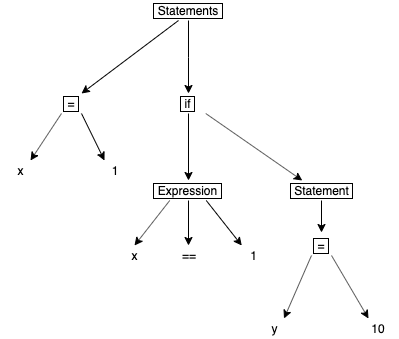
\includegraphics[width=\linewidth/2]{report/images/ast.png}
	\caption{Simple \gls{ast} of x=1; if (x == 1) \{y = 10;\}}
	\label{fig:ast}
\end{figure}



\section{False positives and false negatives}
As stated above, most of the design principles are hard to detect violations of. Because one is not totally sure that sure that a design principle is violated our tool will report violations, that isn't. These are false alarms and we call these \textit{false-positives}. We often discuss the rate of false-positives, which is an important metric to evaluate the usefulness of different rules. We generally would like the rate of false-positives to be as low as possible. It is believed that the higher the value of the rule, the higher false-positive rate we can accept. 

A \textit{false-negative} is the opposite, when actual violations goes undetected. We want to keep this rate as low as possible. 

\section{Code review}
\label{code-review}
Code review is a manual inspection process of looking through code. It is currently the most common way of finding design issues in code. Code review works very well if done correctly, but unfortunately it is easy get wrong, and is time consuming. 
% why it is easy to get wrong

It is a whole lot of things to consider when doing a code review. Naming a few;

\begin{itemize}
    \item Is the solution following the preferred coding style? Are best practices concerning style, and design principles used?
    \item Is the solution well architected? Is it following the architectural model of the application? Are all the files in the correct modules?
    \item Is the solution following relevant design principles?
    \item Will the changes cause unexpected behavior, and break other parts of the system? 
    \item Is the code understandable? Does all variables, method names, classes express its intent?
    \item Is duplicate code introduced? Is this way of solving the problem the way we prefer it to be in this project?
\end{itemize}

When dealing with large amounts of changed code it is easy to forget some of the bullet points above. The number of false-negatives per changed line usually increases as the number of changed lines in a pull request increases. Especially when dealing with repetitive tasks its easy to overlook issues. Luckily, tools will be able to help us with the first point regarding style and best practices. The rest of the points are currently solved by inspecting the source code. Tools should therefore help us by automating most tasks, such that the manual review is focused on finding design issues that tools are not able to detect. 

By detecting issues during code review design defects will be resolved quicker because the developer can fix the issue right away. And fixing issues right away, saves a lot of time.

\section{Developer workflow}

Developers have their own workflows which they find useful, and a tool for code-analysis needs to fit the workflow to help the developer during development. There exists a number of places where a tool could be executed in the coding phases of development. Common examples include:
\begin{itemize}
    \item While coding (Tool runs continuously as the developer types)
    \item On building the application 
    \item On commit (When one bulk of changes is done)
    \item Before \gls{qa} and code review (Often in a \gls{ci} environment)
    \item Anytime the developer wants to execute the tool
\end{itemize}

Depending on the use case of the tool, the tool executes in different phases. The compiler (parser) would for example execute its code-analysis to find syntax errors on every build. The tool needs to execute at correct point to create the least amount of noise. Reporting issues as early as possible may generally seem like a good idea, but could possibly distract the developer from solving the problem at hand. Especially, if the tool itself creates noise (by introducing false-positives or takes a significant amount of time to execute) reporting issues early in the development phases would annoy the developer. 

Simple and advanced analysis and automatic refactoring options is often included and continuously executed inside more advanced \gls{ide}'s. Examples include data-flow analysis, dead-code detection, null-pointer-analysis and automatic transformation of imperative expressions to functional expressions. Often such analysis will help more than annoy the developer by giving immediate feedback. More resource heavy analysis include dynamic analysis, to find for example performance or security issues. These kinds of tools are typically executed at a later stage, for example before a code review. 

Developers also have their own preferences for workflows and when to execute and use tools. Making a tool configurable or fit in multiple execution points in the development process is therefore often appreciated.

\chapter{Related work}
\label{relatedwork}

% General about tools that is related
To the best of my knowledge, a tool that directly targets detection of violations of design principles, does not exist. There exists a lot of tools for code analysis, PMD\cite{pmd}, SonarQube\cite{sonarqube} to name a two of the most used ones for the Java language. Most of them support detection of violations of style conventions, best practices and finding possible bugs. However, some tools and linters include functionality for detecting violations on a small subset of the design principles. Therefore, developers need to adopt a large suite of tools to only be able to support detection of a few design principles violations. Also, the tools are fundamentally different and have different purpose and supports integration in the development process differently, both with its advantages and disadvantages. The tools are ranging from separate \gls{cli}s, native applications, online services, \gls{ide}s and \gls{ide} plugins. The purpose also varies. Some are used for project level analysis activities, for finding areas in the code base with issues, while other tools are focused at reporting issues at the time of writing or in the \gls{qa} process. 

This thesis is mainly considering two research fields. First, related work on code-analysis regarding detecting design principle violations will be presented. Then other related work and tools related to code review and manual inspection of code will be presented.

PMD \cite{pmd} is one of many tools that calculates multiple metrics to indirectly support detecting design issues. Examples of metrics could be \gls{loc}, \gls{cc} and \gls{nof}. The principle of \textbf{High Cohesion - Low Coupling} is a principle that has support in multiple tools, in the form of calculating a metric, including but not limited to JArchitect \cite{jarchitect} and CodeMR \cite{codemr}. JArchitect \cite{jarchitect} also includes functionality for visualizing  High Cohesion - Low Coupling using a \gls{dsm}. Another example of indirectly detecting design principle violations by using metrics is JArchitect. JArchitect uses the \gls{dsm} to find violations of \textbf{\gls{srp}} by looking at how many different types a class uses. Ndepend \cite{ndepend} calculates the \gls{lcom} value to find whether the class is cohesive or not, and therefore possibly breaking \gls{srp}. 

IntelliJ \cite{IntelliJ} (for Java) and \cite{pmd} has support for detecting violations of the \textbf{\gls{lod}} principle through extensive analysis of the source code.

Detecting similar snippets of code to find violations of the \textbf{\gls{dry}} principle is targeted by many tools including, but not limited to IntelliJ\cite{IntelliJ}, PMD\cite{pmd} and Code Climate\cite{codeclimate}. However, code can violate \gls{dry} without looking similar, and tools that can detect more complicated cases have not been found.  

\todo{See if i can find tools that target other design principles. Look at the design principle list on github.}
Other design principles like \textbf{\gls{isp}}, \textbf{\gls{ocp}} and \textbf{\gls{lsp}} are not targeted at all in tools, but several articles and forum posts on how one can spot violations have been found. Composition over inheritance is tightly related to the \gls{lsp} and \cite{composition-over-inheritance-stackoverflow} has been useful in providing hints. Multiple articles about spotting violations of \gls{ocp} have also been found, and has been useful.

\todo{Find the posts and articles and refer them here?} These have been shown useful in implementing rules that are not targeted in the current set of tools.

Regarding the process of code review, services like Github\cite{github}\footnote{From wikipedia: "..company that provides hosting for software development version control using Git"\cite{github-wiki}} provides useful features and integration with other tools for code review. Especially a tool called Danger\cite{danger} provides the possibility of automating comments on \gls{pr}'s. It supports development of plugins to support different kinds of automation. No tools that support finding design defects have been found, but plugins that enable such development have been found. Most notable are the plugins that enables automatically commenting on issues found using various linters. Examples include the danger-eslint-plugin\cite{danger-eslint-plugin} and the danger-detekt-plugin\cite{danger-detekt-plugin} which enables comments on \gls{pr}'s based on warnings created by eslint\cite{eslint} and detekt\cite{detekt}, respectively. 

\chapter{Methodology}
\label{methodology}
The selected research methodology needs to fit the goal of the study. Therefore, the goal of the study will first be presented. Then the selected research methodology will be presented, and how it contributes to reaching the goal. Then, a more detailed description of the different steps in the research methodology will be provided. 

\section{Goals of the study}

There exists a lot of theory and knowledge on how to design and build maintainable software. The knowledge is used by the developers when writing code, and some of the knowledge could be enforced by tools for code analysis. It helps developers write systems that are maintainable. However, there exists knowledge about design principles that is not used in the current set of tools for code analysis. Design principles is not targeted with the current set of tools, because it is shown hard to detect violations of design principles with a low false-positive rate. The high false-positive rates will create noise and disturbs the developer.

The main goal of the study is to create a tool that help developers adhere to the design principles, ultimately improving the maintainability of code. \todo{(hal: Tror ikke "study" er riktig uttrykk når du bygger et verktøy)} By looking at existing tools, existing methods for \gls{ddpv}, and both advantages and disadvantages of existing developer workflows, we think it is possible to develop an effective tool for \gls{ddpv} without creating significant amounts of noise in the developer workflow. An important sub-goal is therefore to find out how to integrate the tool in the developer workflow to reduce the amount of noise. 

The goals and the sub-goals are summarized below:

\begin{enumerate}
    \item [\textbf{G1:}] Create a tool for \gls{ddpv} to help developers write maintainable code
    \begin{enumerate}
        \item [\textbf{G1.1:}] Create a set of rules for \gls{ddpv}
        \item [\textbf{G1.2:}]Designing a solution for how and where to integrate it in the developer workflow to reduce eventual noise
    \end{enumerate}
\end{enumerate}


\section{Research methodology}
To reach the goals it will be necessary to have practical approach where an innovative product is designed, developed and evaluated. As the goal is to help developers creating more maintainable code, it is also necessary to have a user-centered approach for evaluating the product. A traditional agile user-centered design process would be a normal choice for such development. However, for this study the end product should also provide a general contribution to the research field of improving maintainability of code. The contribution should include what is learned in the process, to see if such an approach could be expanded and put more work into and possibly being a new way of helping developers create maintainable software. The Design Science research methodology fits that purpose. It is presented in (A Design Science Research Methodology for Information Systems Research) \cite{10.2753/MIS0742-1222240302}.

% About the chosen methodology
Design science is a research methodology that focuses on getting knowledge about a domain through development of innovative artifacts. The methodology provides specific guidelines for evaluation and iteration in research projects. The software artifact will be created through a series of iterations that include the following activities; problem identification/understanding and motivation, definition of objectives for a solution, design and development, demonstration/testing, evaluation, communication. Figure \ref{fig:designScience} is taken from Peffers. K \cite{Peffers2007ADS} and shows the process of the design science methodology. 

\begin{figure}[h!]
    \centering
    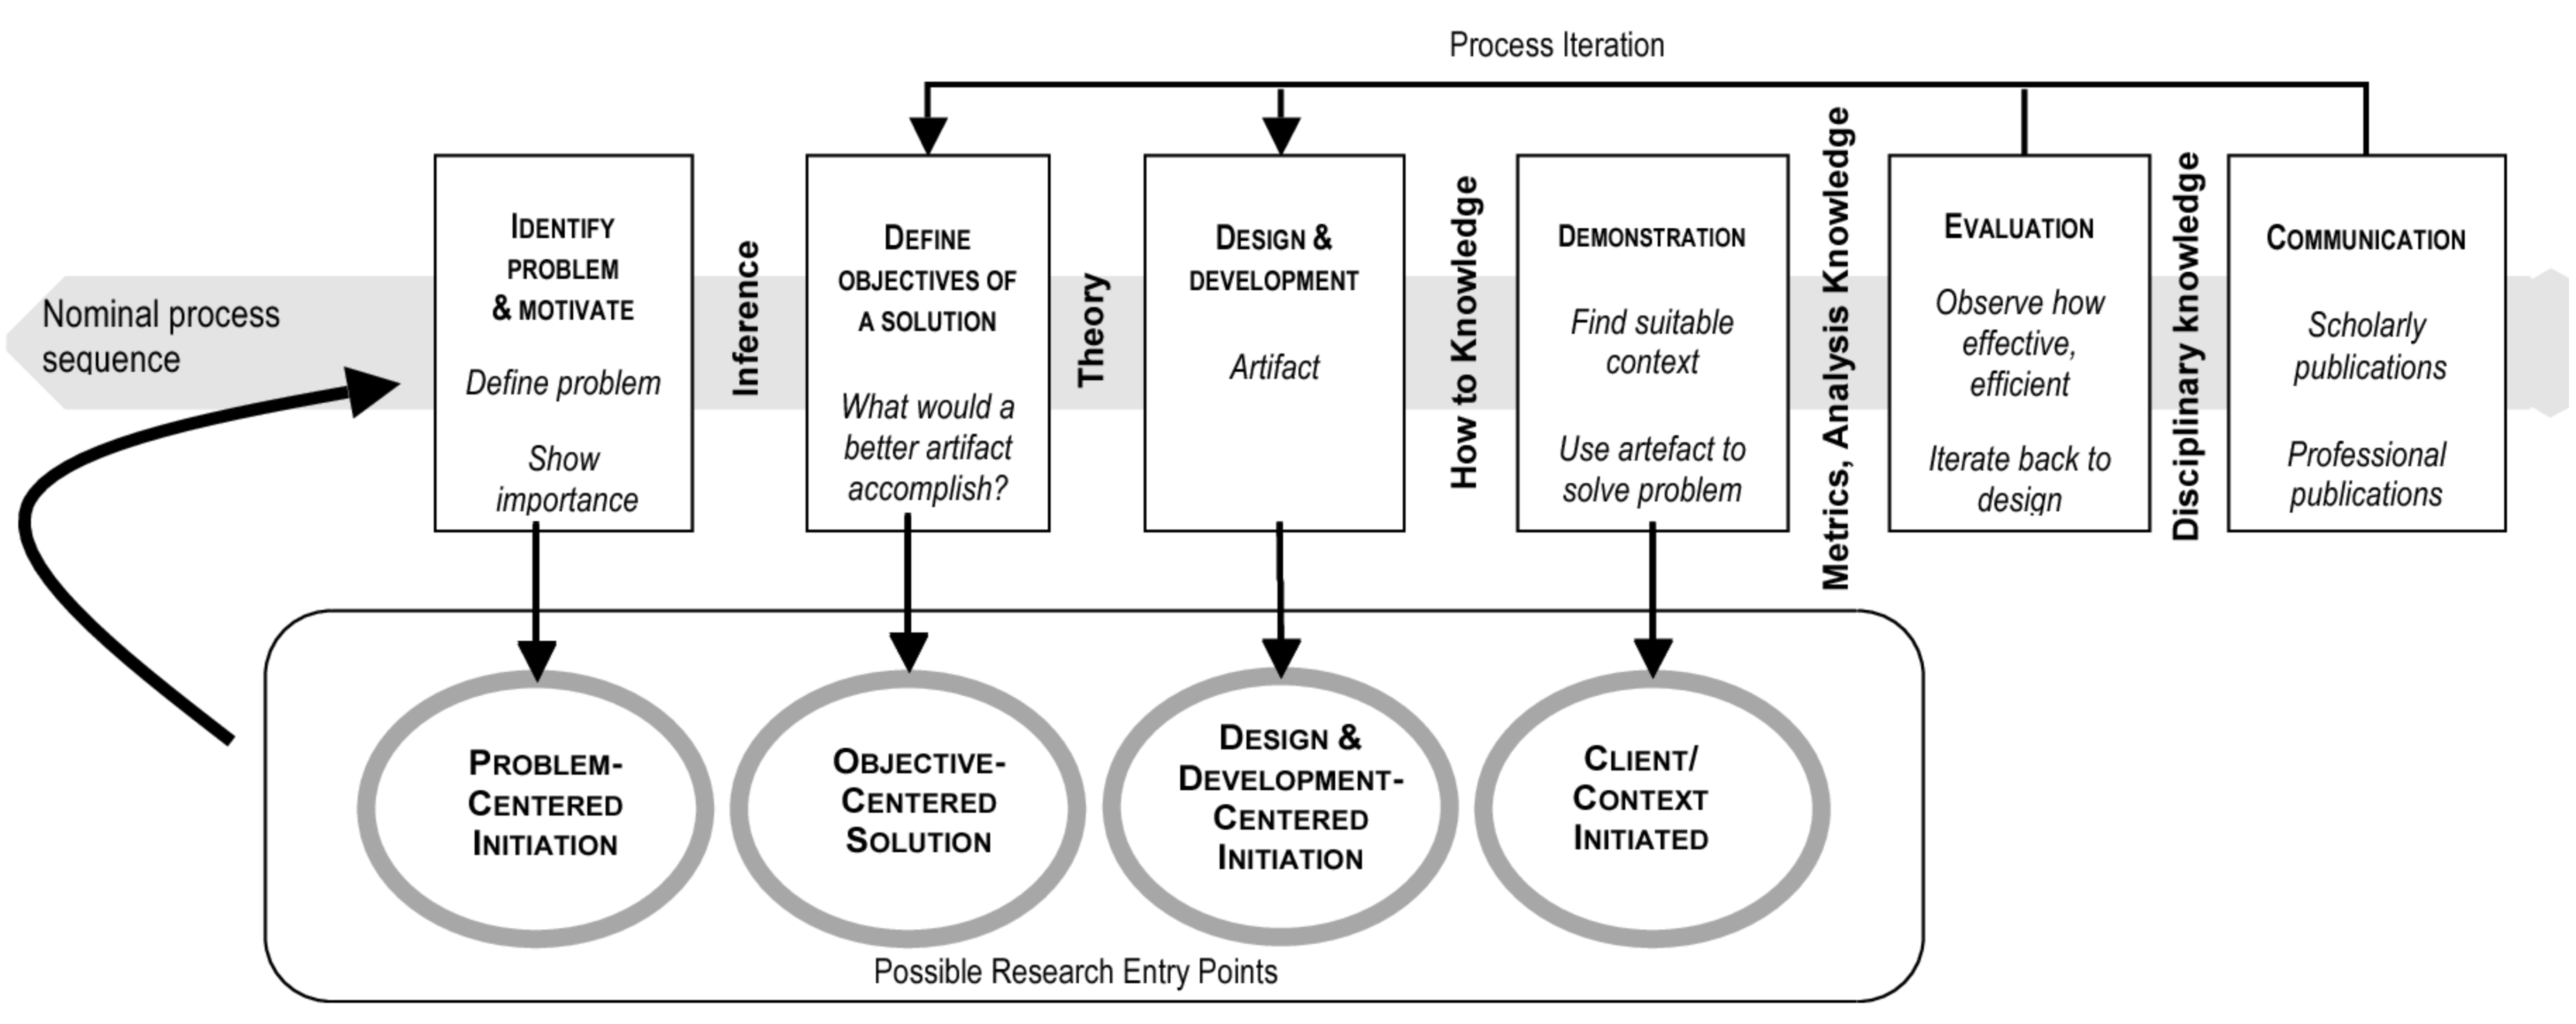
\includegraphics[width=\textwidth]{report/images/designScience.png}
    \caption{The process of the design science research methodology}
    \label{fig:designScience}
\end{figure}

As can be seen in the figure is important to notice that the activities is not done in any particular order, but in that order as seen required. I will elaborate on how the different activities is applied to the study below. 

\section{Problem identification and motivation}
\label{problem-identification-and-motiviation}
\todo{use design issues / design defects consistently}
\todo{hal: Det kommer veldig an på hva du legger i "design"!!! Hvis brukt som "utforming av en løsning for en bruker", som er naturlig i kontekst av "design science", så handler det i høyeste grad også om funksjonalitet. Mens i "design principles" brukes det annerledes.}


% Motivation for detecting design issues is that it is cheaper to develop high quality code
As Martin Fowler explains in his article "Is High Quality Software Worth the Cost?"\cite{is-high-quality-softaware-worth-it}, the common trade-off between quality and cost does not apply to software. High quality software is actually cheaper to produce because "Neglecting internal quality leads to rapid build up of cruft\footnote{Cruft is the difference between how the system is, and how it ideally would be.}, which slows down feature development. Even great teams produces cruft, but by keeping internal quality high, one is able to keep it under control. High internal quality keeps cruft to a minimum, allowing a team to add features with less effort, time, and cost."

The rapid increase in cruft comes from the consequences of neglecting internal quality attributes. As discussed in section \ref{achieving-maintainable-code} an essential part of developing software with high internal quality software is to follow or adhere to the design principles. Andy Glover \& Matt Archer have written an article with 10 arguments why you should fix bugs as soon as you find them\cite{10reasons}, and the same arguments applies to design defects (that is introduced by f.example not following design principles). Below is a short summary of the most important arguments inspired by that article:

\begin{enumerate}
    \item Unfixed design defects may hide other design defects. Fixing the design defects can solve upcoming problems, that would have been harder to find at a later point.
    \item Building upon badly designed software further complicates and increases the difficulty of resolving the issues later.
    \item Unfixed design defects suggest quality is not important. If a software developer is working on poorly written software, it is likely that more code of the same style is added, continuing to degrade the system quality.
    \item Unfixed design defects lead to inaccurate estimates. Having design defects in code will make it hard to modify and extend. New requirements that incur changes to the code base may break unexpected parts of the system. The estimation will then be hard to do.
    \item Fixing familiar code is easier than unfamiliar code. Developers need time to get familiar with code, understand what it does and why. Fixing issues while the developer is in the context of that code will save time.
\end{enumerate}

Therefore, to reduce the cruft, and thereby the cost, we should improve the internal quality which includes following the design principles.


%Developers often fail to communicate the positive correlation between internal quality and development cost, which leads \gls{pm}'s to give internal quality less priority in favor of feature development.


% Motivation for helping the code review
There are mainly two techniques for detecting violations of design principles, code-analysis using tools and manual code-review. Some code-analysis tools offer design principle analysis as mentioned in section \ref{relatedwork}, but suffer from limited functionality regarding design principles and not being integrated into the development process. Therefore, manual code review is the main arena where most design-issues are found. Finding design issues through code review is time-consuming and requires deep understanding of the problem that is being resolved. This process is prone to errors and overlooking due to the nature of human failure. Having a tool that could help this process would help both the reviewer and the reviewee with not overlooking possible design issues, and could cause useful design discussions within the team.

% Motivation for designing a solution for integration with the workflow
Another aspect of such a system is how it should be integrated with the development process to reduce the amount of noise from false positives. If such a system could be created it could possibly be an inspiration for other tools supporting other programming languages or domains that are subject for analysis. \\

\\ The definition of the specific research problem is based on the two main challenges in this study. It is as following: \textbf{How to create a tool for \gls{ddpv} that is integrated in the developer workflow without suffering from noise by false-positives?}

\todo{Does there exist other domains that does involve analysis, but that does not utilize all the information and is suffering from false positives? }

\section{Define objectives of a solution}
\label{objectives-of-solution}

The initial objectives of a solution are based on current knowledge about the domain and how the solution should be engineered to best achieve the goals. 

The first objective is that the solution should be able to detect violations of design principles using static code analysis. As discussed in the background, static code analysis is best suited for this task as we search to improve the source code itself, and not dynamic quality aspects of the code. The selection of principles to support should be based on knowledge on which principles that are most important, and which principles that fits code analysis best. 

The second objective is that the solution should be designed to reduce eventual noise from false identifications. This is based on the knowledge that current tools suffer from false-positives and that implementations have have been skipped or dropped because they created too much noise. By designing the solution to accept and reduce the amount of noise, more design principles could be considered for implementation.

The third objective is that the tool is configurable to fit individual or team preferences. We know that each developer and teams has their own workflow, and to fit them the tool should be configurable, both at the rule-level and at tool-level. Rule-level meaning that it should be possible to select which rules to enable, and tool-level meaning that the tool should be possible to integrate in multiple types of developer workflows.

The fourth objective is that the tool should be included in a existing tool or should be easy to integrate with existing tools. This is based on the knowledge that getting users to adopt a new tools is easier if it is easy to start using, and if others are already using it. It would also drastically reduce the effort required to develop a tool because a framework for code analysis is already provided. 

The objectives of a solution is summarized below:
\begin{itemize}
    \item [\textbf{OS1:}] It detects violations of design principles through a set of rules using code analysis.
    \begin{itemize}
        \item [\textbf{OS1.1:}] Most important design principles considered first.
        \item [\textbf{OS1.2:}] Design principles that fits code analysis should be given priority.
    \end{itemize}
    \item [\textbf{OS2:}] The solution is designed to reduce eventual noise from false identifications. 
    
    \item [\textbf{OS3:}] It is configurable
    \begin{itemize}
         \item [\textbf{OS3.1:}] To fit individual or team preferences on where to use the tool in the workflow. \todo{hal: Er det ikke litt risikabelt å si at dette er konfigurerbart. Hvordan skal man f.eks. kunne konfigurerer det til å skje i IDE-en og ikke ved commit til felles repo? Marius: Verktøyet kan kjøres fra kommandolinjen eller etter PR er opprettet i Github. Ved å legge til "file-watchers" i IDE skal man også få til å kjøre det hver gang en fil lagres. Å få det til å kjøre kontinuerlig i IDE blir noe vanskeligere.}
         \item [\textbf{OS3.2:}] To select which rules to analyze, and possibilities for configuration to support even less false-positives.  
    \end{itemize}
    
    \item [\textbf{OS4:}] It can either be included into existing tools or is easy to integrate with existing tools so that adoption of the tool is easy.
\end{itemize}

As the development progressed, multiple iterations of development, demonstration and evaluation contributed to a better understanding of the problem and objectives was   therefore added or changed. During development of the vertical prototype it appeared harder than initially thought to create and develop accurate rules. A specification of OS1 was therefore made. 

\begin{itemize}
    \item [\textbf{OS1.1:}] It detects violations of \textbf{important} design principles through a \textbf{limited} set of rules using static code analysis.
\end{itemize}

During presentation of the horizontal prototype there was found out that reported violations should include context of the code (referring to actual constructs in the code) to ease the process of deciding if a detection is a true- or false-positive or to help with the solution. 

\begin{itemize}
        \item [\textbf{OS5:}] Reported violations includes code context to ease the process of deciding if it is a true- or false-positive. 
\end{itemize}

Later on, it was discovered that the performance of the application was bad due to bad optimization of the developed rules. A new objective for a solution was therefore defined:
\begin{itemize}
    \item [\textbf{OS6:}] Good performance
\end{itemize}




%It all boils down to time=\$. The tool will only provide value of we can save development time using it. Then, if the sum of time saved by finding design issues earlier is more than the sum of the negative impact of considering the false-positives, the tool will provide value.
%As a general objective we can say that, the tool will provide value if the value of detecting true-positives is worth more than the negative impact of all the false-positives. 
%However, to measure the time spared by detecting issues earlier is an impossible task to measure, but we know that it is quite


Rule specific objectives: 
Comments are understandable, and provides suggestions for solutions.

\section{Design and development}
\todo{usecases, requirements ?}


% Generally about design and development
The design and development phase involves the development of vertical- and horizontal prototypes, with high and low resolution, as well as the final artifact. 

% Theory about prototypes
\textit{Horizontal prototypes} covers a broad view of the entire system and focuses more on user interaction with the system, rather than low level details. \textit{vertical prototypes} on the other hand focuses on the technical challenges and a single functionality of the system. Depending on the precision, or how much it looks and works like the finished product, it is either a \textit{low resolution} or \textit{high resolution prototype}. 

First, low resolution prototypes will be created, and then more high resolution prototypes. The reason is that we want to get feedback on the initial idea as quick as possible and to adjust the product accordingly. Why and how the different artifacts was created is written about in the results section for each of the product artifacts.
 \todo{write about tdd?}
\section{Demonstration}

% General about demonstration. Specific demonstration details is found in results section.
The next logical step after developing a prototype is to demonstrate and test it. Depending on the prototype created, different forms of demonstration will be used. Examples include functional testing and presentation of prototypes. The most important aspect of demonstrating the prototypes, is to create an environment that is as similar as possible to the environment that the final product will be used in. A so called field test. This involves getting users (other developers) to test the prototypes and the final product. The user group that is best suited for being informants are experienced developers that have knowledge about applying and using design principles.

%Unfortunately, because a lack of resources and funding on the research project they were impossible to recruit for more in-depth evaluation. Attempts at recruiting informants for in-depth testing of the product was done by having presentations, posting on social media, creating posts in developer forums, and posting in chat groups for related tools and for work, without any luck. Additionally, the corona virus disease made physical recruitment more difficult. A conscious decision on shifting the focus to internal evaluation and feedback from open-source community was therefore seen necessary.

\todo{By creating \gls{pr}'s in open-source projects and advertising the tool through backlinks to the repository on GitHub, more feedback could be gathered. Analysis of old \gls{pr}'s in public projects could also be done to give results that could be evaluated manually. }

A specific description of how the demonstration of each prototype was done can be seen in the results section.
\todo{tried to get feedback by: posted in slack channels work work, kotlin etc, updating the readme for better seo and to show off the product, creating Prs in muliple repositories to advertise. creating issues in related repositories., reddit, hackernews.}

 
\section{Evaluation}
% General about evaluation. Specific evaluation details is found in results section.
In the evaluation phase we will observe and measure how well the developed artifact solves the problem. We will compare the artifact with the objectives of a solution, and use different techniques for evaluation based on the type of artifact and at which stage in development we are. Evaluation methods includes qualitative methods and quantitative methods. The qualitative methods include feedback gathered from having conversations with experienced developers and through presentation of prototypes. The quantitative methods include interest measurement and analysis of efficiency of the final artifact.   

The methods were mostly informal as formal methods were impossible to organize. This is a major flaw of the study and is targeted in section \ref{flaws-of-study}. Informal evaluation methods were easier to organize and caused useful discussions, possible features and useful feedback. 

Continuous evaluation of the prototypes and the developed artifact is important to adjust the product to the users needs. After each evaluation activity, based on how the artifact compares to the objectives of a solution it is decided if another iteration is required. The results from the evaluations is presented in the result chapter.

\section{Communication}
The end result and the developed knowledge about \gls{ddpv} is diffused in this master thesis, for others to consume. It should provide a general contribution to the research field of improving the maintainability of code through code analysis. It should communicate the results and provide insight in what could be improved and areas subject for more research. The final artifact is available for use and further development on GitHub\cite{detekt-hint-repository}.

\chapter{Results}
\label{results}
Describing the exact number of iterations and the iteration steps is not possible as one continuously evaluates the product and adjusts the product under development. But seeing the development process in a big picture we can approximately look at 4 iterations in the design science methodology. A visualization of the general process can be seen in figure \ref{fig:workflow}.

\begin{figure}[h!]
    \centering
    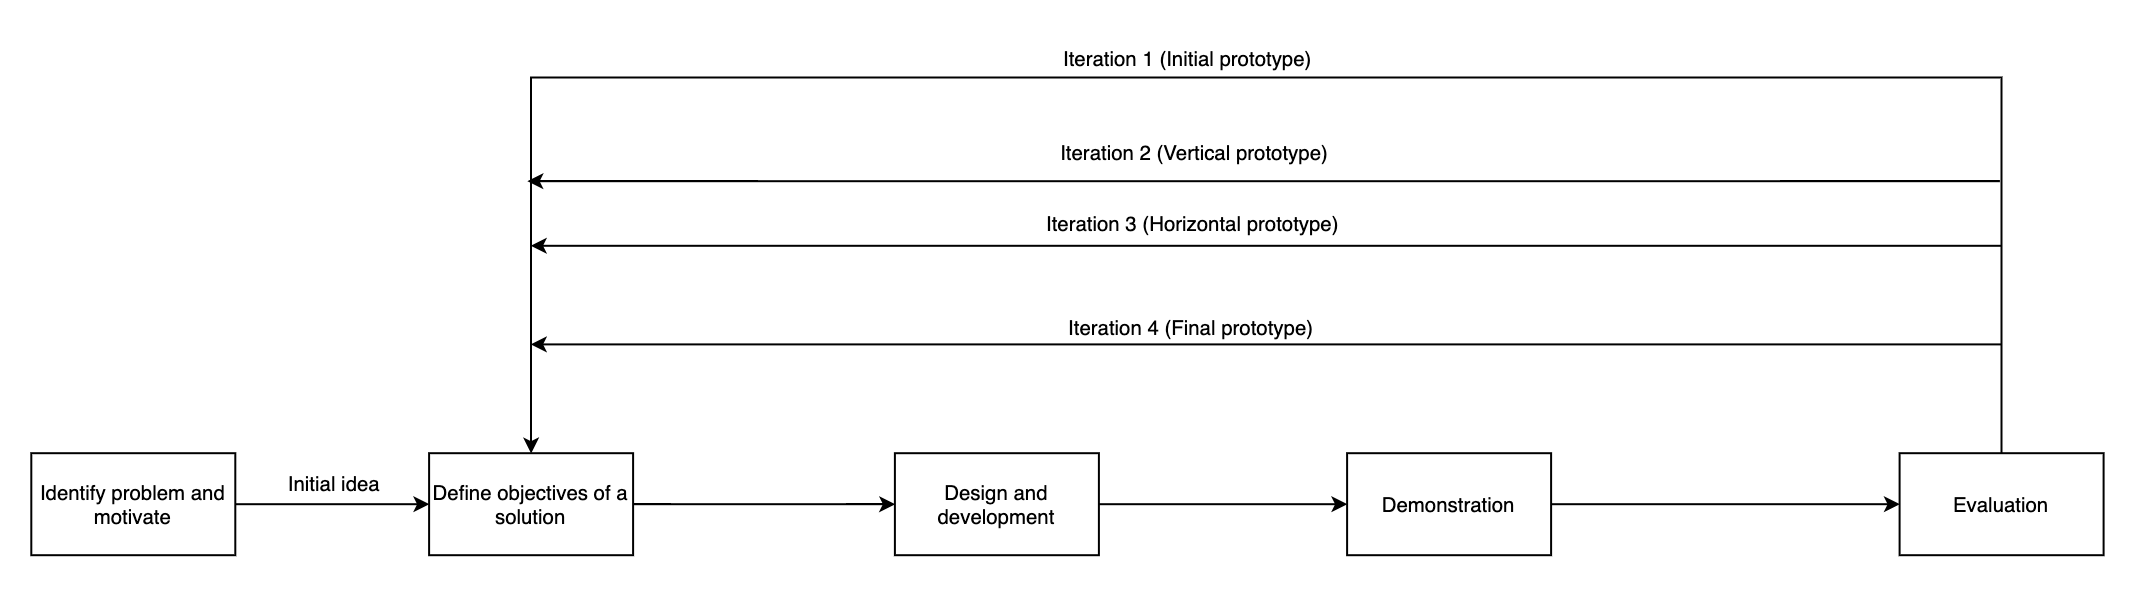
\includegraphics[width=\linewidth]{../images/workflow.png}
    \caption{The general process of developing the final artifact}
    \label{fig:workflow}
\end{figure}

The 4 iterations were focused on 4 different versions of the product. The different versions are described and their evaluation are described in the next sections. The results are presented it the order they were achieved, making the next section a result of the previous one. A description of the technical solutions and details is found in section \ref{technical-solution}.

\section{Initial prototype}
\subsection*{Why and how it was created}
An initial low resolution prototype was created to see if there was any interest in a tool for detecting design principle violations. The initial idea proposed a design where the tool would report design principle violations by posting comments directly in the \gls{pr}. The prototype can be seen in figure \ref{fig:mockup}. The prototype was focused at finding a solution to \textbf{OS2} (The solution is designed to reduce eventual noise from false identifications). By having a tool that is executed just before code review, it will not cause any disturbance in early stages of development. False-positives would be easy to ignore and would not require any action to get rid of. Similar tools require effort in suppressing errors, either by polluting the code base with annotations or adding issues to a whitelist/blacklist file. In addition, commenting on \gls{pr} will only add comments to changed lines of code, reducing the amount of warnings that will appear.  

\begin{figure}[h!]
    \centering
    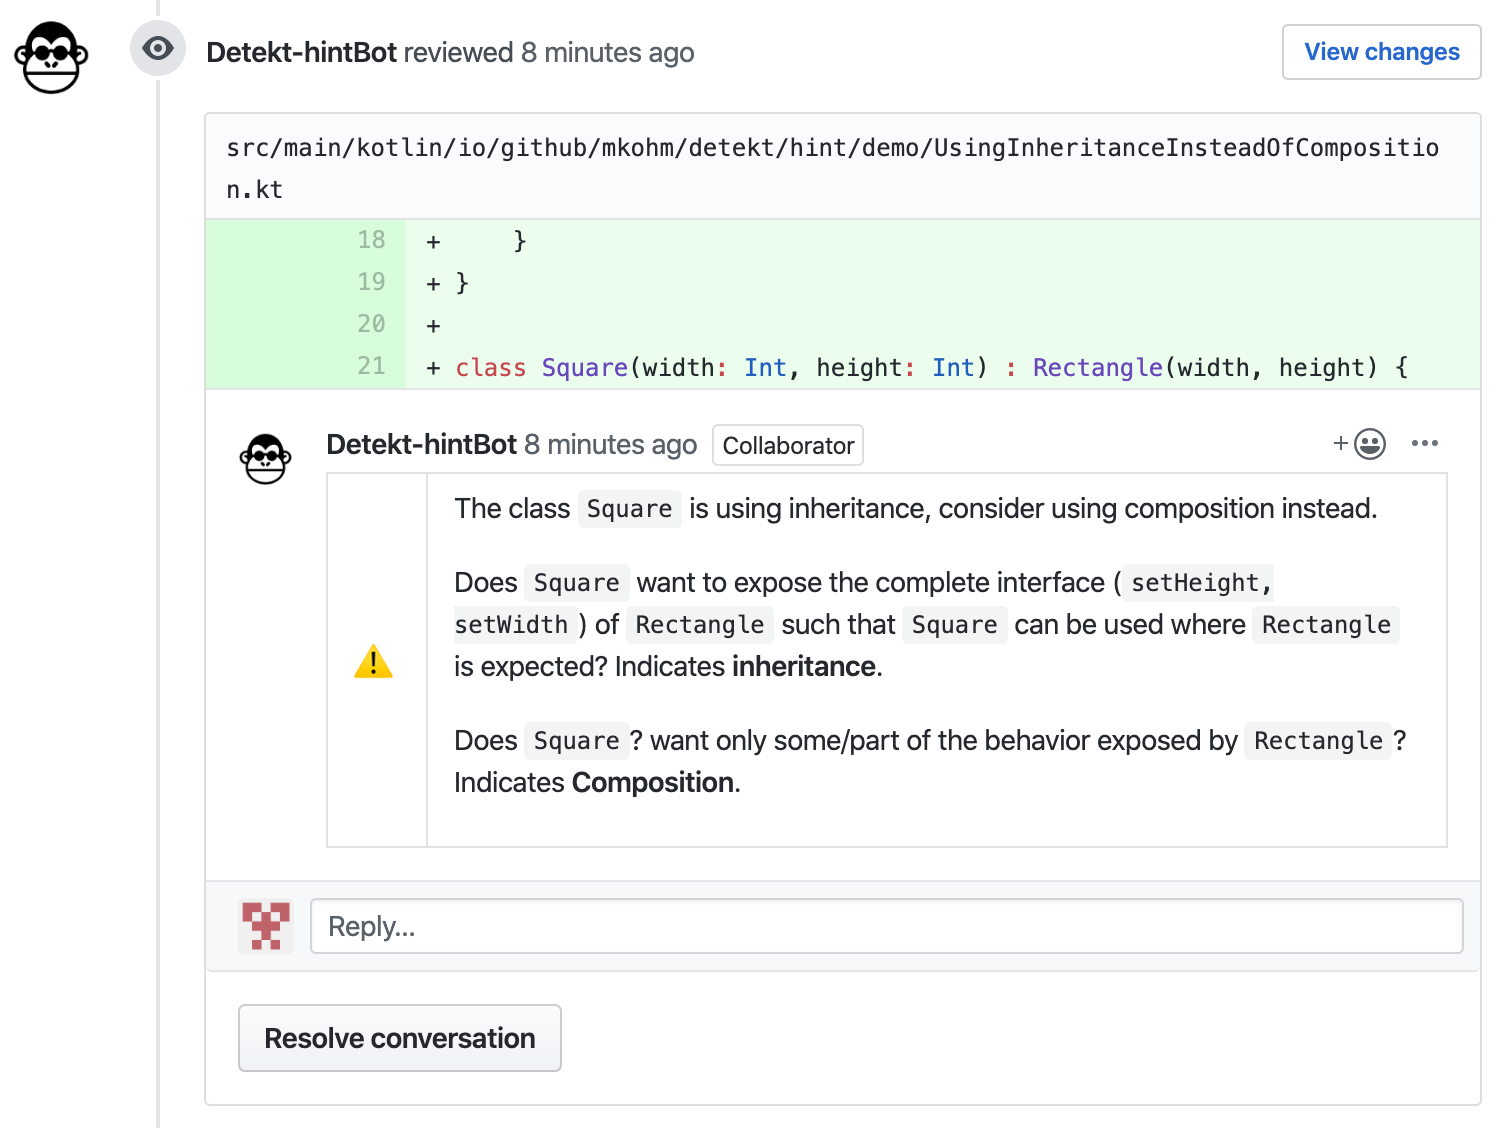
\includegraphics[width=\textwidth]{../images/demo.png}
    \caption{Initial prototype that was presented on social media}
    \label{fig:mockup}
\end{figure}

\subsection*{Demonstration}
The initial prototype was posted on the subforum of Kotlin\cite{kotlin-reddit} and SoftwareArchitecture\cite{softwarearch-reddit} on Reddit. Additionally, the prototype was presented and discussed with friends. 

\subsection*{Evaluation}

The general feedback was that there was an interest in a tool like this, and that it would solve some of the issues with false-positives. However, some did still point out that reducing the amount of false-positives still would be one of the most important focus points. Other suggestions for improvement included: 
\begin{itemize}
    \item Do not claim that the developer is wrong when there can be a lot of false-positives, instead present it as it \textbf{might} be a violation of a design principle, and guide the developer to taking the correct decision.
    \item Identifications and even false-identifications could create useful discussions within the developer team.
    \item Focus on removing the amount of false-positives as much as possible and making the product configurable to fit different needs.
\end{itemize}

This feedback was only based on discussions with friends and a handful of comments in the forum threads, and a fair amount of upvotes. In both subforums, the post received an amount of upvotes that made the post "top this week" in under 12 hours. However, the actual value of the feedback may be limited. Read more about this in section \ref{flaws-of-study}. 

\section{Vertical prototype}

\subsection*{Why and how it was created}
The initial prototype proposed more work into creating a tool for detecting design principle violations, and using automated comments during code-review to reduce the amount of noise from false-positives. Normally, a vertical prototype is built first, with the intention of getting an idea of which features that needs to be implemented and the priority of those. In this case a vertical prototype was built first for three reasons:

\begin{enumerate}
    \item The prioritization is somewhat known up front. Being a product focusing on detection of design principle violations, it is quite natural that the product should prioritize principles that are not covered by other tools and that the most significant principles are considered first.
    \item Too see if building a tool for detecting design principle violations is a feasible task within the scope of a master thesis.
    \item Developers tend to be more interested in technical solutions that is working than non-interactive prototypes. Getting feedback on the following horizontal prototype would be easier if actual solutions to technical problems could be presented.
\end{enumerate}

% How the prototype was created
Before building the prototype an in depth investigation of different approaches was done. The tool would ideally support multiple languages, but to limit the scope and because of interest and knowledge about Kotlin and its ecosystem, it was selected as the language subject for analysis. Several tools and frameworks was considered to use as the fundament for a tool, including Ktlint\cite{ktlint} and Code Climate\cite{codeclimate}, but Detekt\cite{detekt} was chosen as the best platform to build on because it was made extensible, and plugins for detekt was already existing for the automated \gls{pr} tool\cite{danger-detekt-plugin}, Danger\cite{danger}. Therefore, Detekt looked as a promising alternative for fulfillment of the objectives of a solution described in \ref{objectives-of-solution}, but a prototype needed to be built to confirm that assumption. 

\subsection*{Demonstration}
The prototype was mainly demonstrated and continuously evaluated during development to the developer. It was also partly presented to the participants at the detekt-hint presentation at Javabin Trondheim.

\subsection*{Evaluation}
Evaluation of the vertical prototype is based on the objectives of a solution, and a evaluation of the applicable objectives is presented below.
\begin{itemize}
    \item [\textbf{OS1:}] Using Detekt as a platform, we are able to write detection-rules by analysis of the Kotlin \gls{ast} by using the Detekt rule framework and the  Jetbrains \gls{psi}. Using the detekt \gls{api} was a highly manageable task due to good documentation and a large amount of sample rules to look at. The analysis itself using the Jetbrains \gls{psi} \gls{api} was shown to be more difficult and time consuming. It involves programming in a complex environment with a huge API with lack of documentation. In addition, creating inspections for programming languages involves handling a lot of edge-cases that can take time to cover. Writing test cases for all the different scenarios ensured the proper handling of edge-cases. As development progressed the \gls{api} got more manageable and looking into other platforms or solutions for analysis were therefore not considered.   
    
    \item [\textbf{OS2:}] By using the danger detekt plugin, violations reported by the detekt plugin can be commented on pull requests, exactly as proposed in the initial prototype. The noise will therefore be significantly reduced. In addition, rules can be written with high accuracy using the detekt-api, the amount of false positives can be held to a minimum. 
    
    \item [\textbf{OS3.1:}] Provides possibility to configure tool to fit mainly two workflows. Can be run separately using the \gls{cli} or running the Gradle task to analyze the whole code base, or be used directly in the code review by using the Danger integration.
    \item [\textbf{OS3.2:}] Provides configuration options for rules through the use of a configuration file so the rules can be configured to fit the developers or teams best. The configuration file can contain configuration of, but is not limited to threshold values for rules and excluding files for analysis based on exclude patterns. 
    
    \item [\textbf{OS4:}] The tool is easy to use with detekt, as the developed tool is a detekt plugin. It is However, to use the tool with the Danger integration it requires some additional setup files, creating a bot user on Github and integration with the \gls{ci} environment. This is not an optimal solution, and approaches looking to improve this should be considered. All the tools and plugins that are used are open-source, making it possible for everyone to adopt the tool.
    
    \item [\textbf{OS5:}] Code context can easily be added to comments, by getting the required information from the code-analysis and posting comments that is formatted with markdown.

\end{itemize}

The prototype therefore solves many of the objectives of a solution. However, because of being a prototype it only supported 1 rule that had a lot of false positives, and evaluation of the actual usefulness of the tool could not be performed. In general, it was a successful prototype that was a proof of concept and laid the foundations to further development. The main takeaways from evaluating the prototype:
\begin{itemize}
    \item Detekt is a good platform for building such a tool and enables fulfillment of most objectives for a solution.
    \item Running the tool on own and others code is a good way of finding possible bugs and false-positives.
    \item Further development should focus on a small set of the most important rules, because they can take a long time to implement. And further evaluations of the tool need to address the usefulness of it.
\end{itemize}

\section{Horizontal prototype}
\subsection*{Why and how it was created}
As the vertical prototype showed; a limited number of rules have to be supported. That raised the question of which rules to implement and how they should support the developer in taking correct design descisions. Looking through a lot of principles, i tried to determine which rules that would be useful. Based on the feedback from the inital prototype, the comments were written in a way that were providing guidance instead of claiming changes because of violations. Since \gls{solid} is considered by many to be the most important set of design principles, the focus was put on those. I also wanted to test out if a visual representation of violations of design principles and solution is preferred or significantly better than a textual representation. The process ended by creating the horizontal prototype that included the rules that i had the most value. 


The horizontal prototype was built by creating sample \gls{pr}'s in a sample repository on Github\cite{sample-repository}, and then commenting on the \gls{pr}'s with the bot user. An example from the prototype is presented in figure \ref{fig:liskov}.

\subsection*{Demonstration}
Initially, to get structured feedback on the prototype, it was planned to present the prototype to a group of people using a semi structured interview. To get informants to the semi-structured interview, a presentation for approximately 20 participants at Javabin\footnote{A usergroup for persons interested in software development on the Java and \gls{jvm} platform, and related technologies.} Trondheim was held. Search for informants also included asking companies with Kotlin developers, including Bekk and Netlight, but with limited success. 6 \todo{inkluderer eirik, kanskje en fra netlight?} participants signed up for joining the semi-structured interview, but i were only able to get in touch with 2 of them to actually join the semi structured interview. The interview followed the semi-structured interview schema that can be found in the appendix \cite{}.

Due to the outbreak of \gls{covid19}, physical meetings could not be arranged, and further complicated the issue of contacting and speaking with other developers directly. I was then forced to find other ways of reaching out to people to gather feedback. The prototype were shown in multiple slack channels for work, the official Kotlin channel and various other channels.


\begin{figure}[h!]
    \centering
    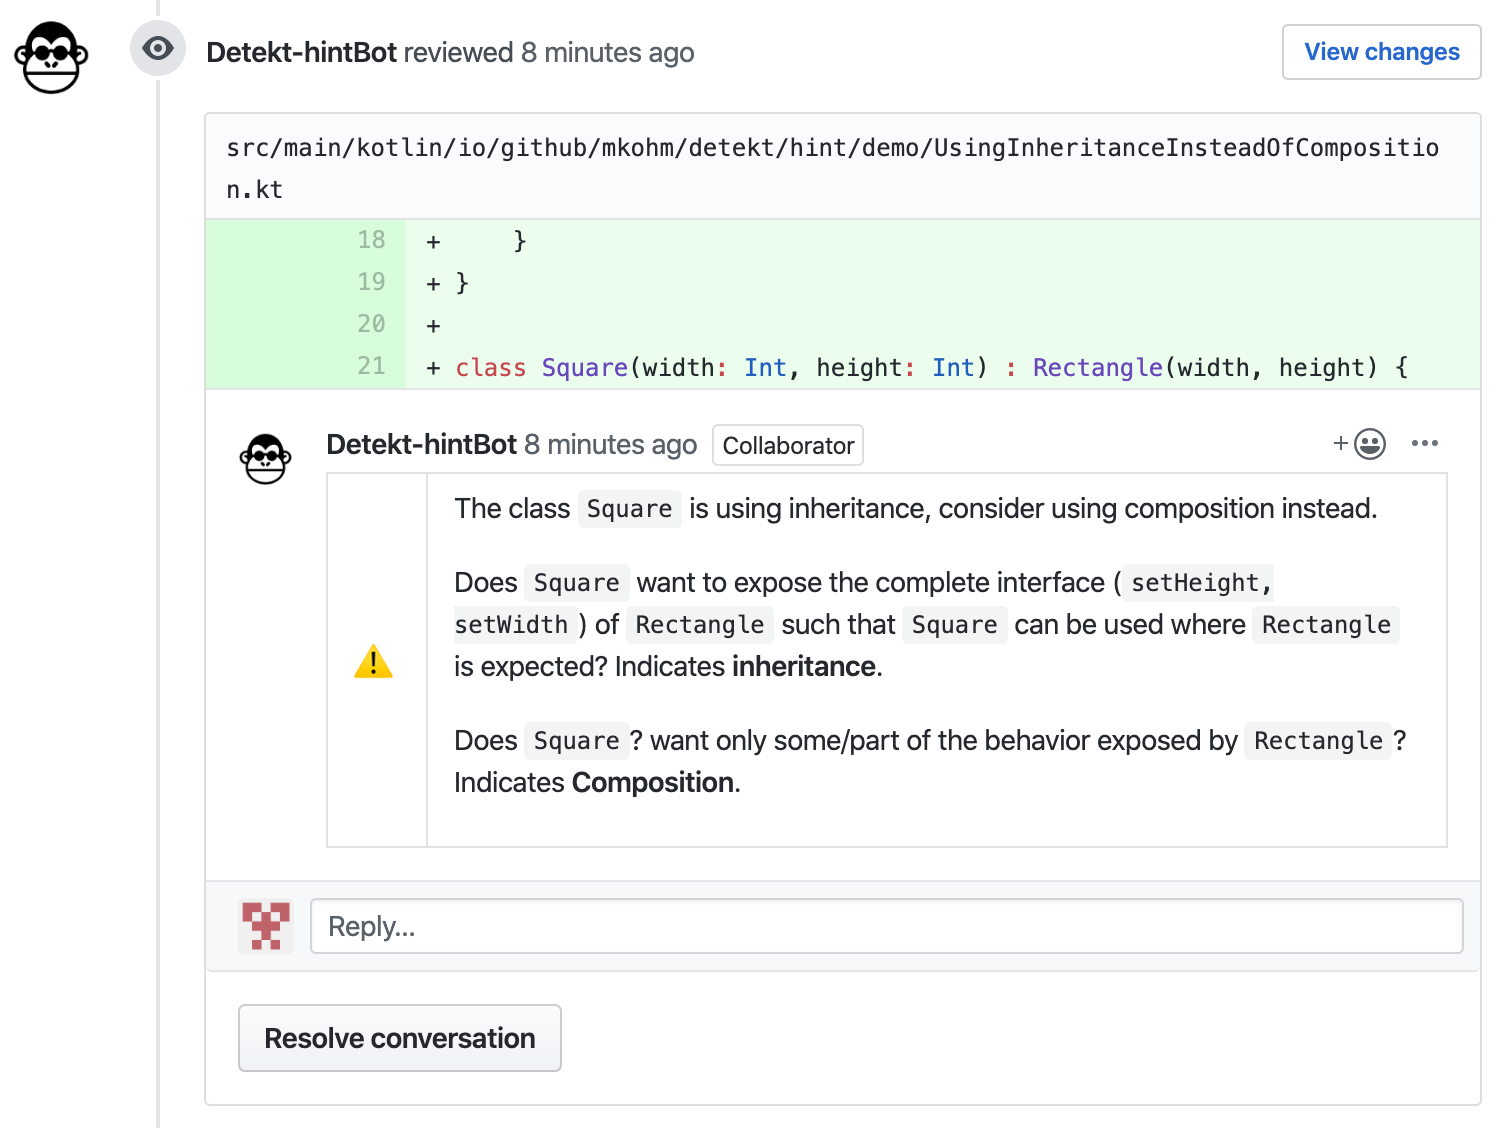
\includegraphics[width=\textwidth]{../images/demo.png}
    \caption{Screenshot of horizontal prototype - Showing the composition over inheritance / \gls{lsp} rule}
    \label{fig:liskov}
\end{figure}


\subsection*{Evaluation}
\todo{can i include images from slack? To proof that i have done some effort in recruiting and getting feedback?}
From the semi structured interview it was found out that visual representation of design principle violations was showing useful, especially when including refactoring hints, but would act more as showoff than provide more value. The implementation costs of generating such images was higher than the value of visual representation. More rules should be prioritized instead, and a textual representation of refactoring possibilities would be almost just as good. There were also a concern related to too few rules implemented, and that the tool would give limited value because of too few issues reported. 

From other ways of demonstrating the general impression was much of the same as for the initial prototype. People like the project, and are generally positive. However, very few suggestions for improvements or others design principles to support were suggested.

The schema used for the semi-structured interview, the participants answers/feedback and selected images of the prototype can be found in appendix \ref{horizontal-prototype}. The full prototype can be found in the sample repository \cite{sample-repository}. \todo{clean up there}



\section{Final artifact}
\subsection*{Why and how it was created}
The final artifact is a continuation of the work done in the vertical prototype, and hence has the same qualities and ways of solving the objectives of a solution. A more technical in depth description of the final artifact is found in section \ref{technical-solution}. Because of feedback on visual representation of violations it was instead decided to provide refactoring possibilities trough a textual representation. A focus on implementing more rules was also done. 

Because earlier approaches for feedback gave limited amounts of feedback, it was decided that a next approach needs to include a functional prototype that would detect actual design issues in code.


\subsection*{Demonstration}
Through a workshop, where participants analyze their own Kotlin code with detekt-hint the final artifact was supposed to be evaluated. However, a new approach for evaluating the artifact had to be considered. A supporting-tool for collecting merged \gls{pr}'s, and analyzing them needed to be created. 


Analysis of pull requests and see if we can find some issues. \todo{write about how covid19 affected this}
Schema:
%Who is the participants, some background information on them. What did the participants say. What is the takeaway from the workshop? What did i change in the product after having the workshop? Because of difficulties related to finding informants, i had to focus on evaluating the prototype by myself, and gethering numbers for how many 

\subsection*{Evaluation}

compare the end result with the objectives of a solution.
\begin{itemize}
    \item false-positive rate / per rule
    \item how many comments per PR avg? How obtrusive is the tool? How much noise does each rule create? Is this less noise than linters create? Linters may need suppressions of rules etc.
    \item How easy to integrate? Many lines of configuration, multiple files and stuff?
    \item How performant is it? How long does it take to run? Is that good enough?
    \item Does it target all the most important design principles?
\end{itemize}

What is the goal, how should i reach the goal of the workshop. Keep the workshop structured.


Gather a group of Kotlin/Android entusiasts for a workshop where one could order pizza and code using this tool. Focus on feedback. Could for example analyze some code that they know and give some feedback on whether it is useful or not. What would have been useful?


\section{Technical solution}
\label{technical-solution}

The developed solution is a static analysis tool that gives the developers guidelines or hints on how to follow design principles. Following is a description of the different components and ending with a description of how they interact with each other.


\subsection{Detekt}
Detekt is a static analysis tool for kotlin. Detekt is comprised of a set of rules for analysis of Kotlin source code. Part of Detekt is also the detekt-api, which gives access to a framework for creating rules, configuring rules, and for analyzing the source code. Under the hood it gives us access to IntelliJ \gls{psi} for code analysis. The PSI is built on top of the \gls{ast} provided by the Kotlin compiler, and enables modification, querying and navigation of the underlying \gls{ast}. Detekt is made extensible, and plugins (with new rule-sets) can easily be added.   

Figure \ref{fig:psi} shows a simplified example \gls{psi} that detekt-hint would use to find violations of \gls{isp}. The analysis would simply look in the PSI for classes that implement interfaces, and see if the overridden methods of that interface are empty or only throws exceptions. 

\begin{figure}[h!]
    \centering
    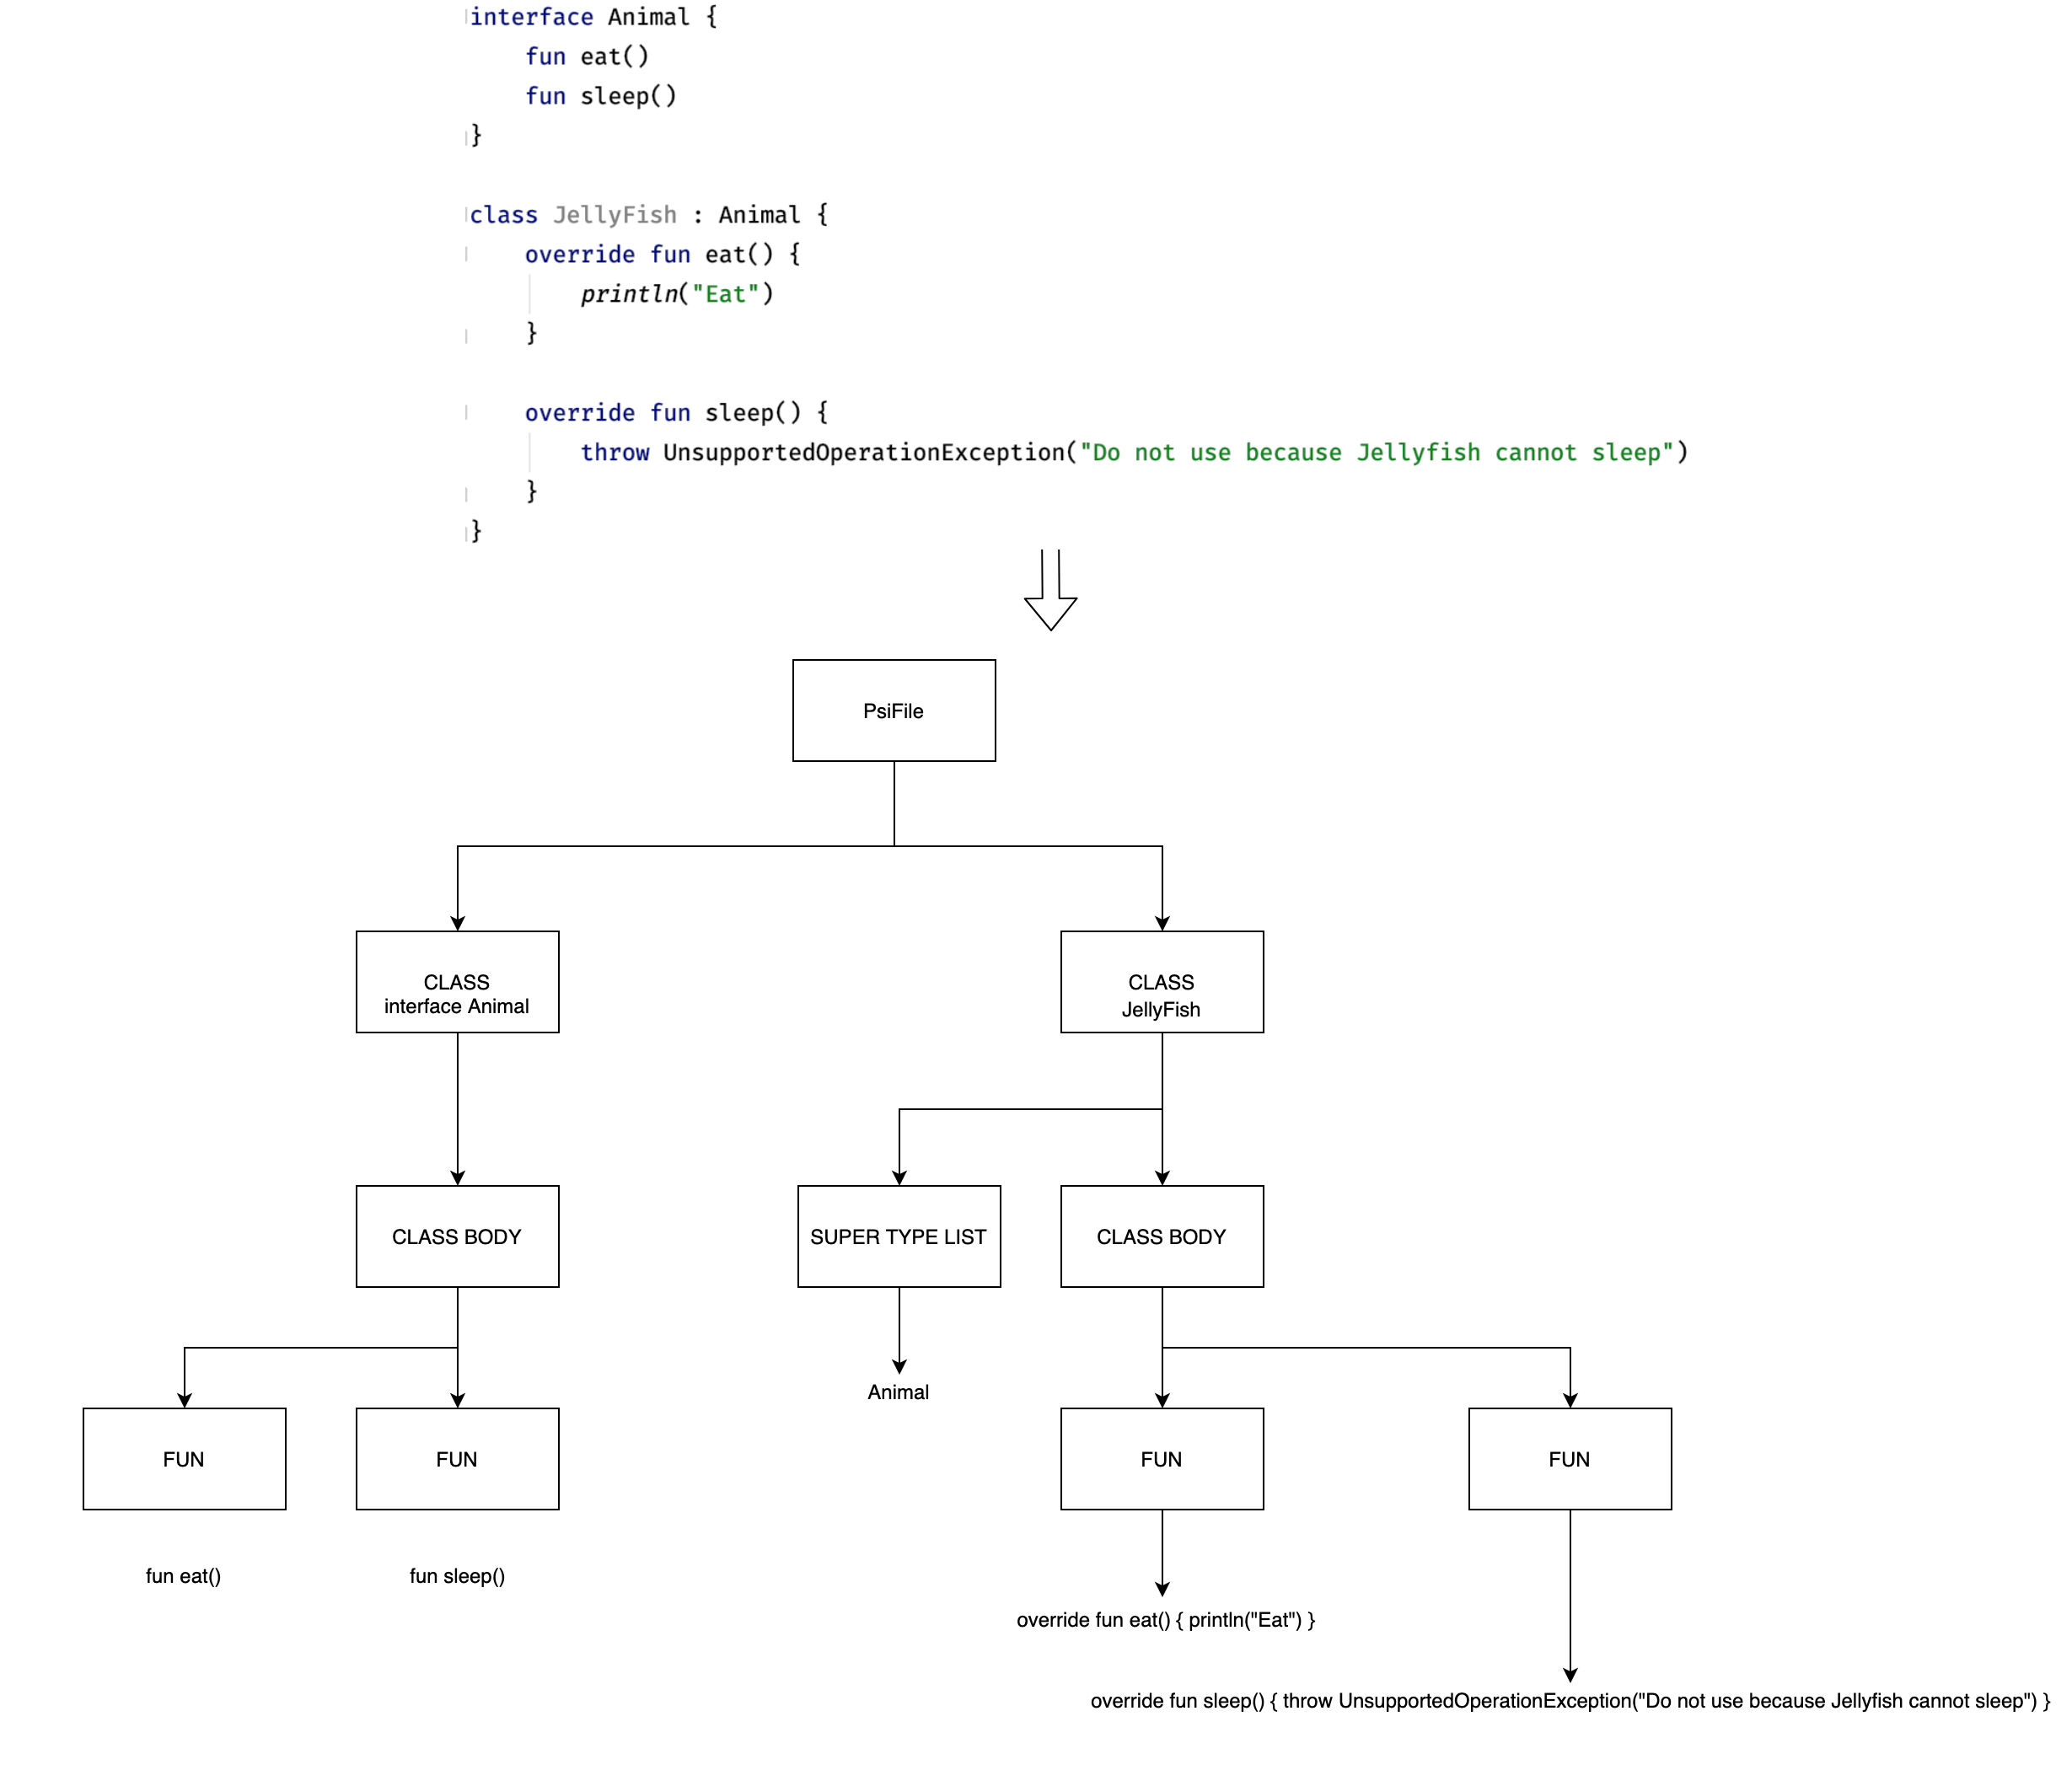
\includegraphics[width=\linewidth]{report/images/psi.png}
    \caption{Simplified version of a sample \gls{psi} showing a sign of violating the \gls{isp}}
    \label{fig:psi}
\end{figure}

When detekt is running, it looks at all the implemented rules (and the configuration of them) and does analysis of the source code. When issues are found, the line number is noted, together with the comment to be added, and added to a report, which is the final output of the program. 

\subsection{Detekt-hint}
A plugin for Detekt is exactly what detekt-hint is. It is a new rule set that can be added to detekt. What is different from Detekt is that it creates rules with more context and is integrated with Danger to support showing issues directly in the \gls{pr}.

\subsubsection{Detekt-hint specification}
The final artifact consists of \todo{enter number} rules. Below follows a technical description of the implemented rules.
\begin{itemize}
    \item Use composition over inheritance (Liskov substitution). The rule will fire when inheritance is introduced, and help test for Liskov substitution. The rule will not fire if you derive from a class that exists in a third party package. This will reduce the amount of warnings created where the framework or library are forcing you to introduce inheritance.         
    \item Lack of Cohesion Of Methods (LCOM). A rule that notifies if there is too much lack of cohesion. LCOM for a class will range between 0 and 1, with 0 being totally cohesive and 1 being totally non-cohesive. For each property in the class, you count the methods that reference it, and then you add all of those up across all properties. You then divide that by the count of methods times the count of properties, and you subtract the result from one\cite{}.
    \item Interface Segregation Principle (\gls{isp}). A rule that looks for classes that implement methods it does not need. It looks for classes that implement interfaces and that contains either empty methods, or methods that only throws exceptions.
    \item Open-Closed-Principle (\gls{ocp}). A rule that looks for instance of checking and switching on enums. It is a common sign of violating the Open-Closed Principle. Will not warn when checking on instances provided by a third party framework or library.
\end{itemize}

%Final source code can be found on Github\cite{detekt-hint-repository}. Developed as a plugin to detekt. Is built as a jar and either included in the gradle build script as a detekt plugin or run separately as a command line interface.

\subsection{Danger}
Danger is a system which is created for the purpose of commenting directly on \gls{pr}'s. It provides an easy to use \gls{api} for extracting the required information from git, and provides methods for commenting directly on pull requests. It is run in your \gls{ci} environment on every commit to pull requests that is made. When the rules are adhered to, the comments are amended to reflect the current state of the pull request. Danger is extensible through the use of plugins.

\subsection{Danger detekt plugin}
The Danger-detekt plugin is a simple plugin which takes a gradle task which is executing detekt. The generated report from Detekt is parsed and comments on the \gls{pr} is added.

\subsection{Integration}
In a proper setup, everything is set up to run within the \gls{ci} environment. First, Danger is executed. Danger runs the Danger-detekt-plugin which runs the specified gradle task for running detekt on the repository. Since detekt-hint is added as a ruleset to detekt, the rules from detekt-hint will be executed and a report containing issues will be generated. The Danger-detekt plugin will then parse the results and output the results in the form of comments on \gls{pr}'s. A diagram of how everything interacts with each other can be seen in figure \ref{fig:integration}. 


\begin{figure}
    \centering
    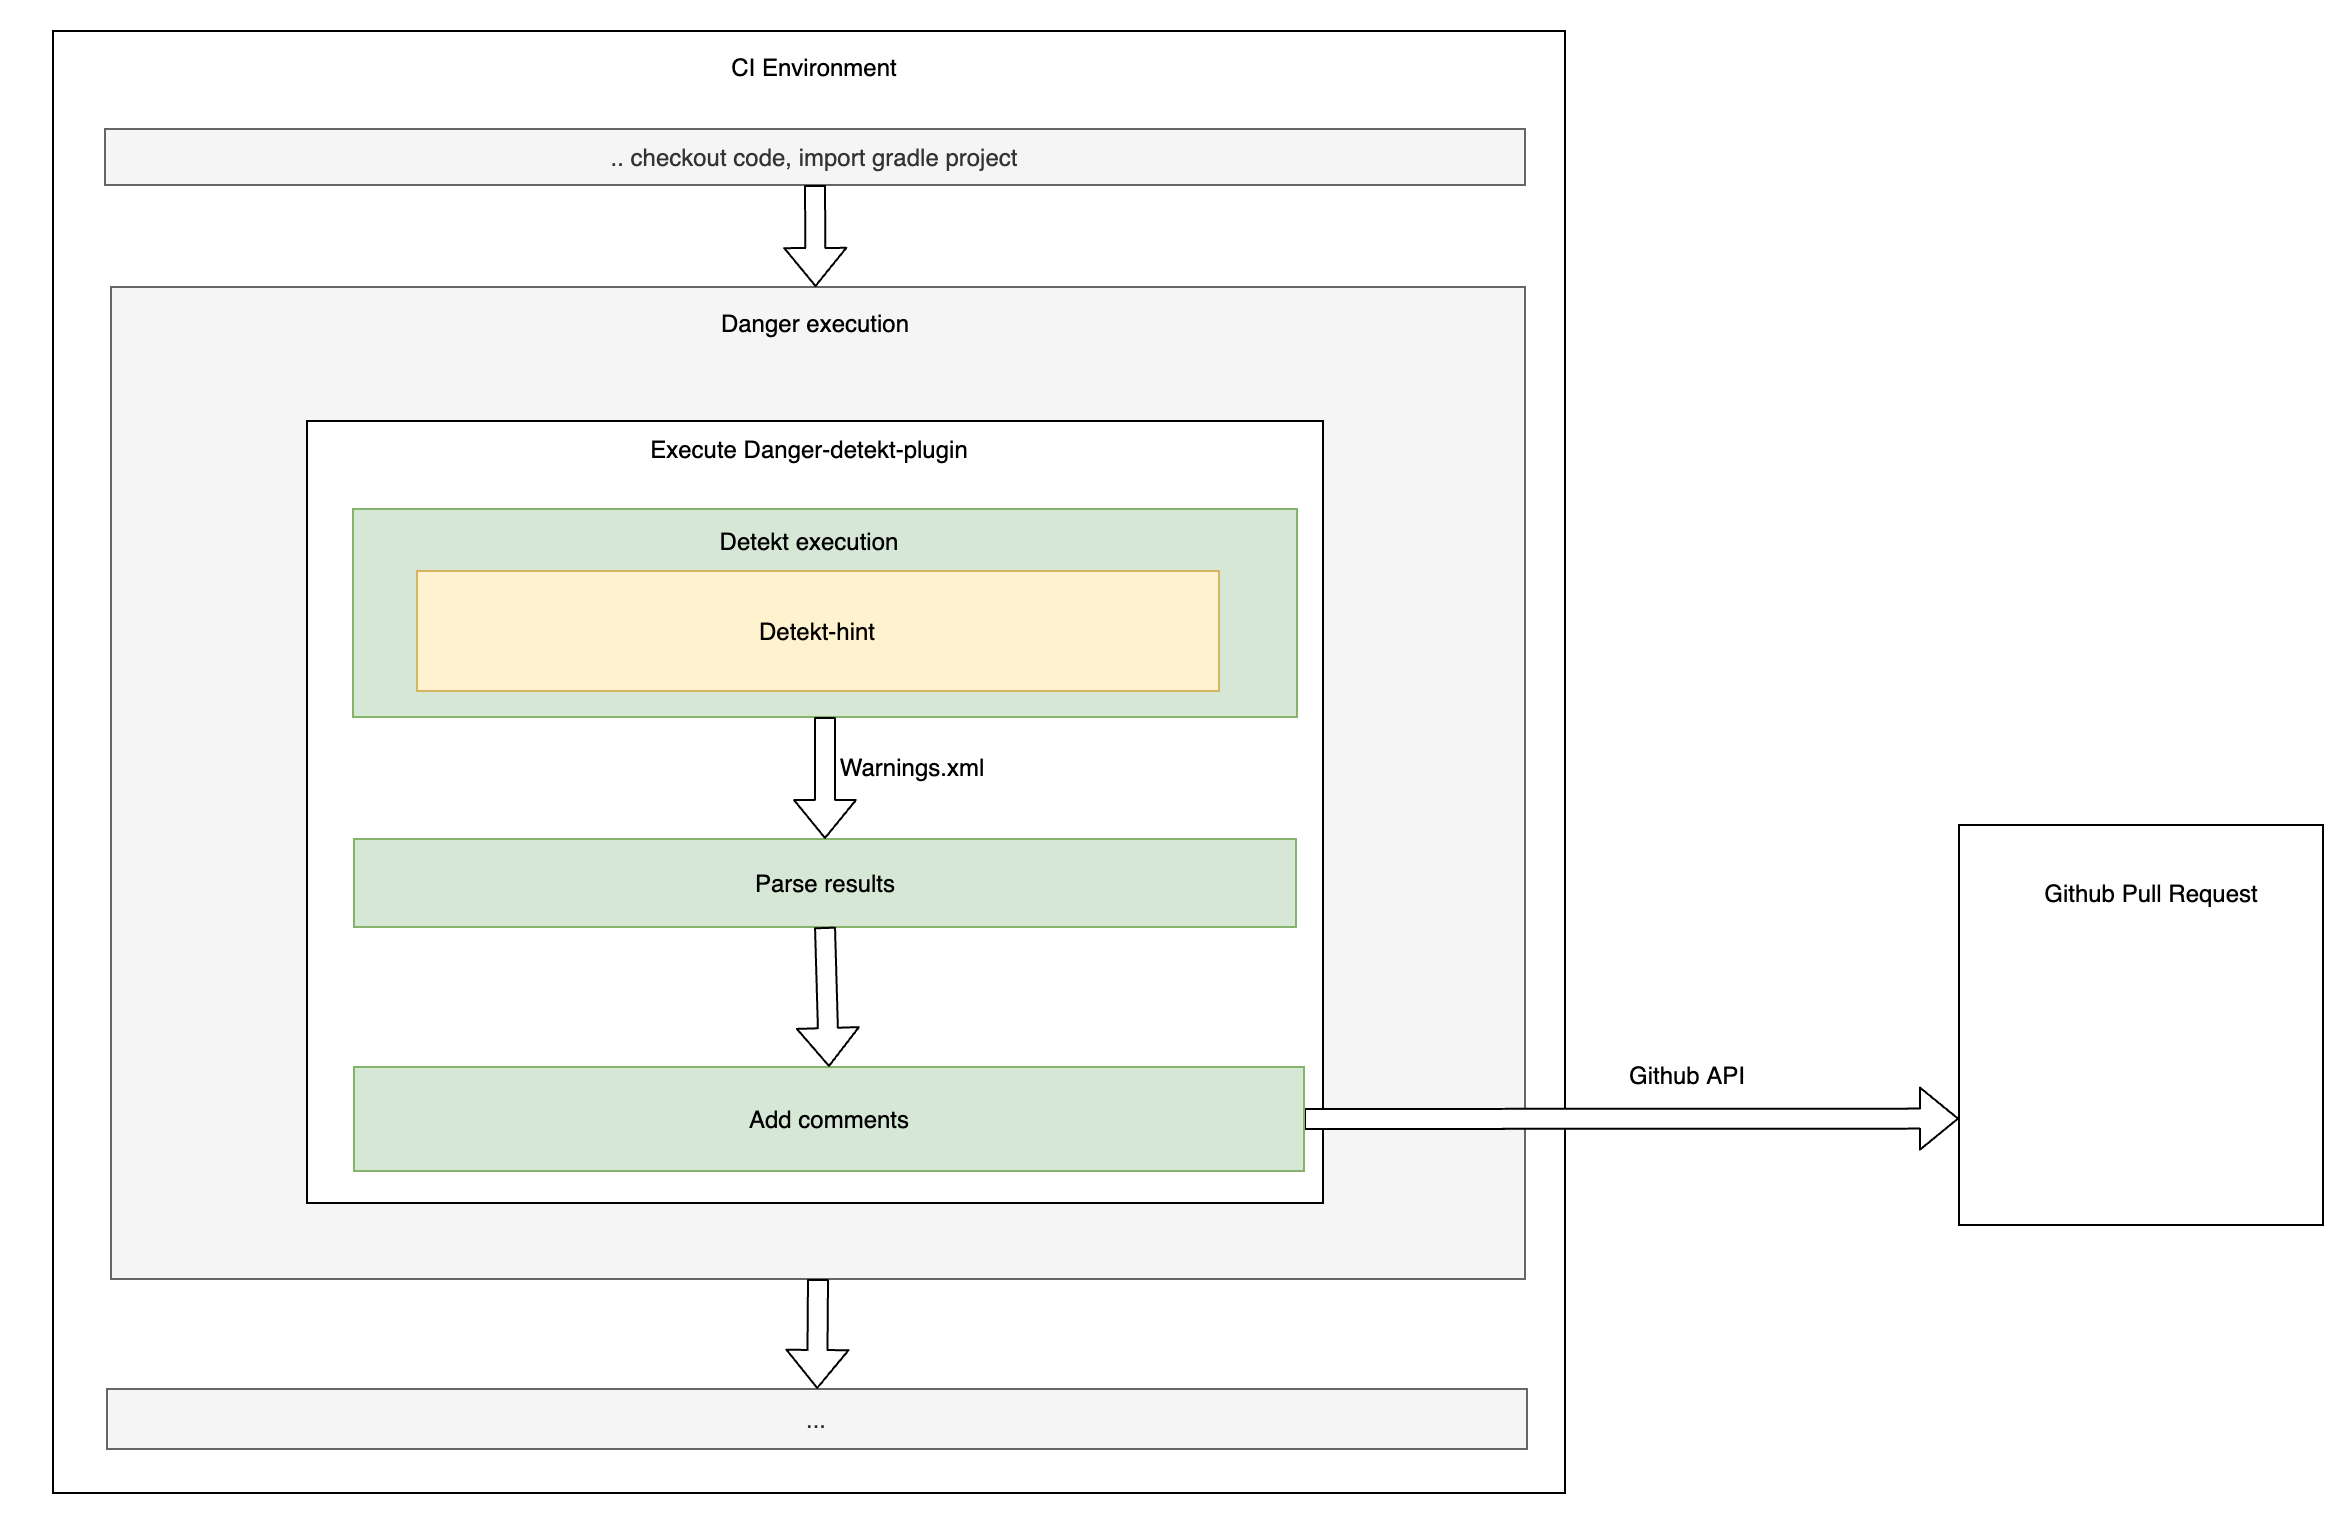
\includegraphics[width=\textwidth]{report/images/execution-flow.png}
    \caption{The overall architecture/execution flow of the solution}
    \label{fig:integration}
\end{figure}


\subsubsection{Getting started}
A setup guide can be found at \cite{detekt-hint-repository}.




\chapter{Discussion and conclusion}
\label{discussion}

\section{Discussion}
Given the results.. 

\section{Future work}
\todo{just say a few sentences about each thing, keep it short and concise.}
There are mainly two ways of continuing the work on the tool, either by improving the current functionality or by extending it with new functionality. 

\subsection{Enhancement}
Lower false positive rates
Enhance the integration/setup process
Enhance the comments, and improving the suggested solutions. Possibly suggesting multiple solutions.
\subsection{New features}
Supporting more more design principles is an obvious way of including more features to the tool. For example ... principle and .. principle. 

Since the tool are able to cope with higher rates of false-positives it is not restricted to targeting only design principles. Other types of knowledge or best practices could be included as rules as well. Other types of rules could involve comments that works as a simple checklist for pull requests. Are tests included? Is coding done blindfolded? Is this file in the correct package/module?    


Look at the evaluation results and fix/work on all of those! 
Implement more rules. More accuraty calculations of LCOM. Considering the different types of LCOM values and choose the best one.
Reducing the amount of false positives.
Announce the tool so more developers would use it.
Rules that show useful with very low false-positive rate should be included into the design section of the mother repository detekt.
Providing more context and/or possible solutions in the comments. Images or graphs explaining.
Increasing the performance.
Easing the setup process. Github app? Direct integration with the repository with no setup. A tool like code-climate that does not need any configuration. Plus of tool like this: all setup is in source control. Downside: could be tedious to set up or not all team members want to use it.
could include other things than design principles, but things that easily is forgotten in code review. blind coding, file organization .... list goes on. everything that is hard to check or easy to forget. 

look at dynamic software metrics, and see how it could be implementet, or if it should get more focus from tool developers, as it looks promising. Dynamic softawer metrics are according to https://www.researchgate.net/publication/225261876_A_Survey_of_Dynamic_Software_Metrics more accurate, and could possibly target design principles in a different way.

\subsection{Adopting the tool}
Getting peopel to adopt the tool through advertisemens etc.

\section{Flaws of the study}
\label{flaws-of-study}
\subsection{Lack of formal evaluation methods}
Formal evaluation methods are better for structured feedback and to find the overall results instead of single users perspective. 

not enough informants - lack of testing the software
informants lacking knowldge about design principles
Should create samples for the horizontal prototype that demonstrates possible false positives as well as true positives. Kan gi inntrykk av at programmet er lurere enn det egentlig er siden jeg bare presenterte de positive identifikasjonene. Inntrykk av interesse på reddit kan være feil pga dette.
not able to gather informants physically, only through digital medium. Easy to ignore, and boring to attend such things. Hard to find experienced developers in Kotlin - that also have the time and will to help out. Without getting anything from it. Limited resources.
\section{Conclusion}
\label{conclusion}
Based on the results, the tool may be useful, but lacks .... More development is proposed.

\section{Acknowledgements}
\label{acknowledgements}
First of all, a big thanks to my supervisor Hallvard Trætteberg for advice, useful discussions and for help in getting in touch with experienced developers. all participants in workshop and prototype sessions.

\printbibliography

\appendix
\label{appendix}
\clearpage
\chapter{Appendix}

\section{Horizontal prototype}
\label{horizontal-prototype-images}

\begin{figure}[h!]
    \centering
    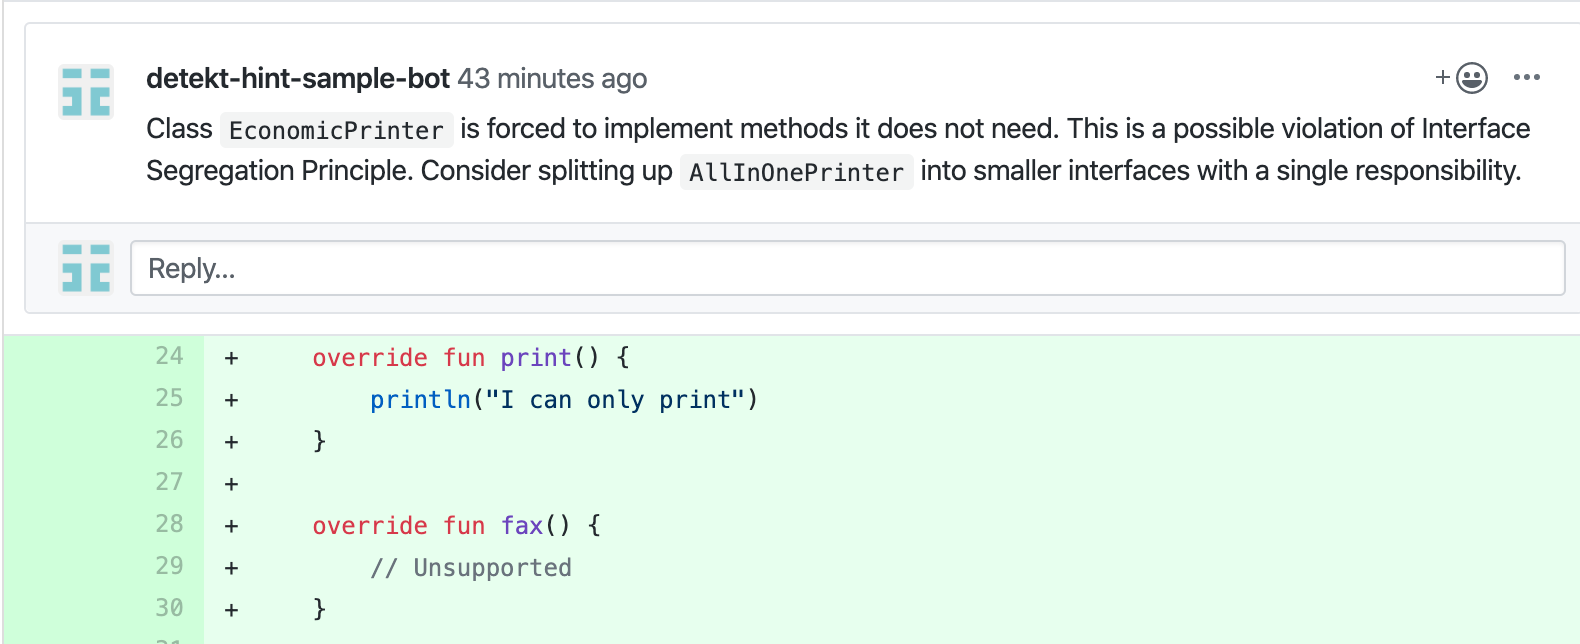
\includegraphics[width=\textwidth]{../images/comment_isp.png}
    \caption{Screenshot of the horizontal prototype showing the \gls{isp} rule. It has detected an empty method, which is a sign of violating the \gls{isp}. In this case the \texttt{EconomicPrinter} implements methods from \texttt{AllInOnePrinter} which it does not need. A solution would be to define separate interfaces for each of the responsibilities (e.g \texttt{Printable, Faxable, Scanable}) and let the concrete implementations of printers implement the interfaces they need.}
    \label{fig:isp}
\end{figure}


\begin{figure}[h!]
    \centering
    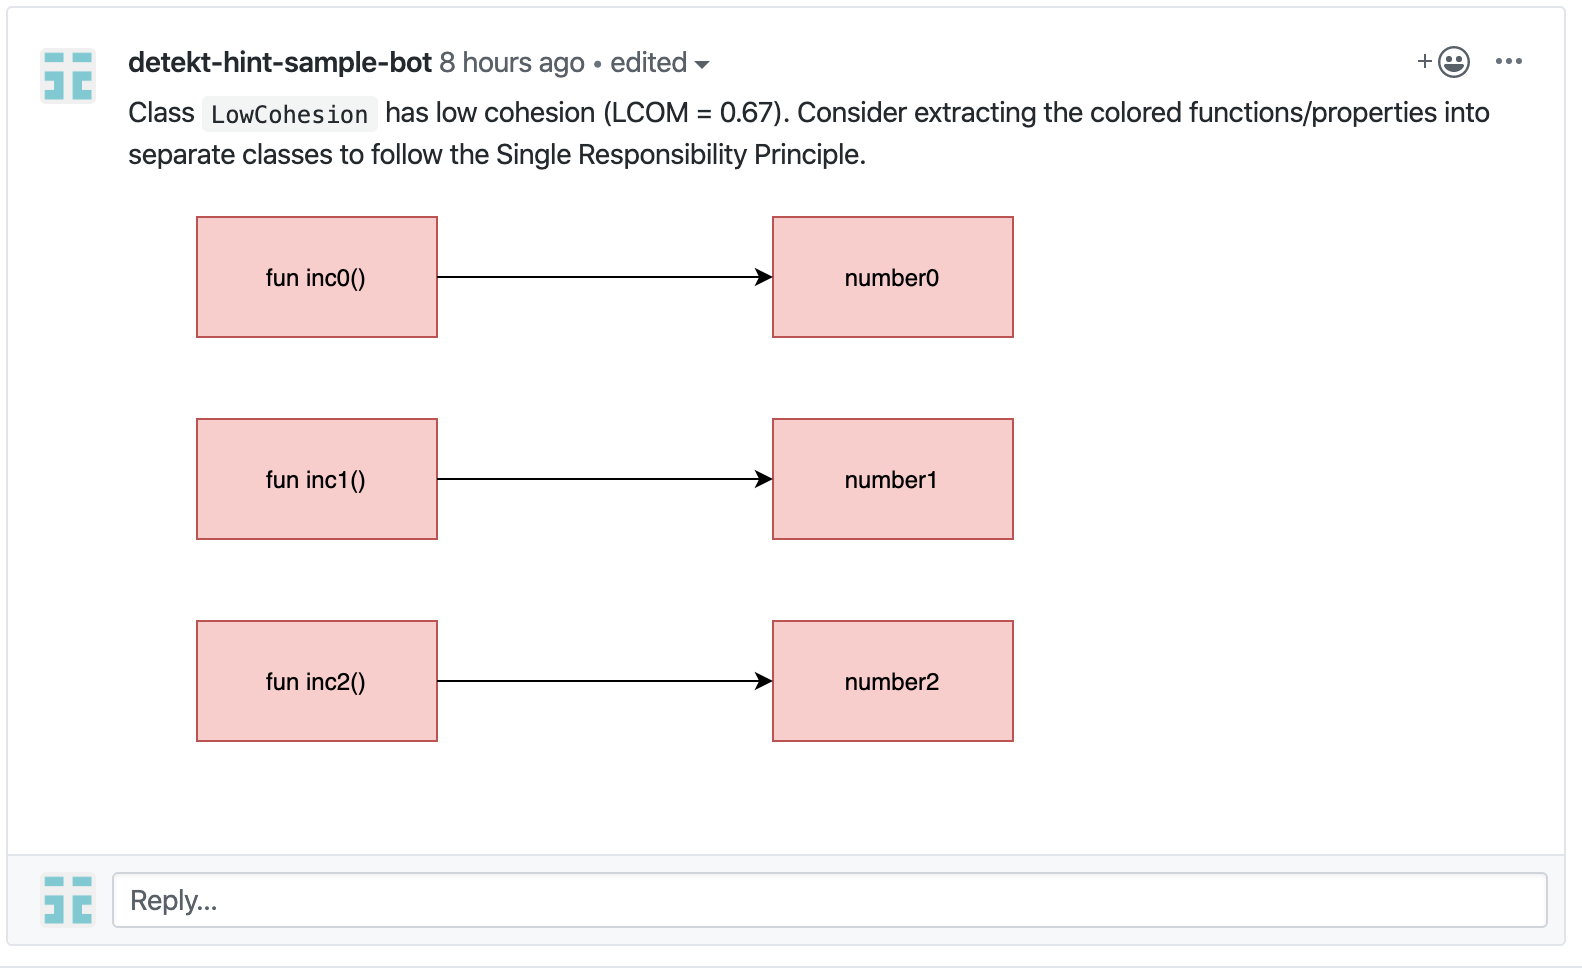
\includegraphics[width=\textwidth]{../images/comment_lackOfCohesion.png}
    \caption{Screenshot of the horizontal prototype showing the \gls{lcom} rule, with a visual representation of the lack of cohesion. The figure shows which fields that are referenced from each of the methods in the class. In this case all the methods of the class references their own separate field. This indicates that each of the methods and corresponding fields have separate responsibilities within the class. This would therefore be an indication of violating the \gls{srp}.}
    \label{fig:lcom}
\end{figure}


\begin{figure}[h!]
    \centering
    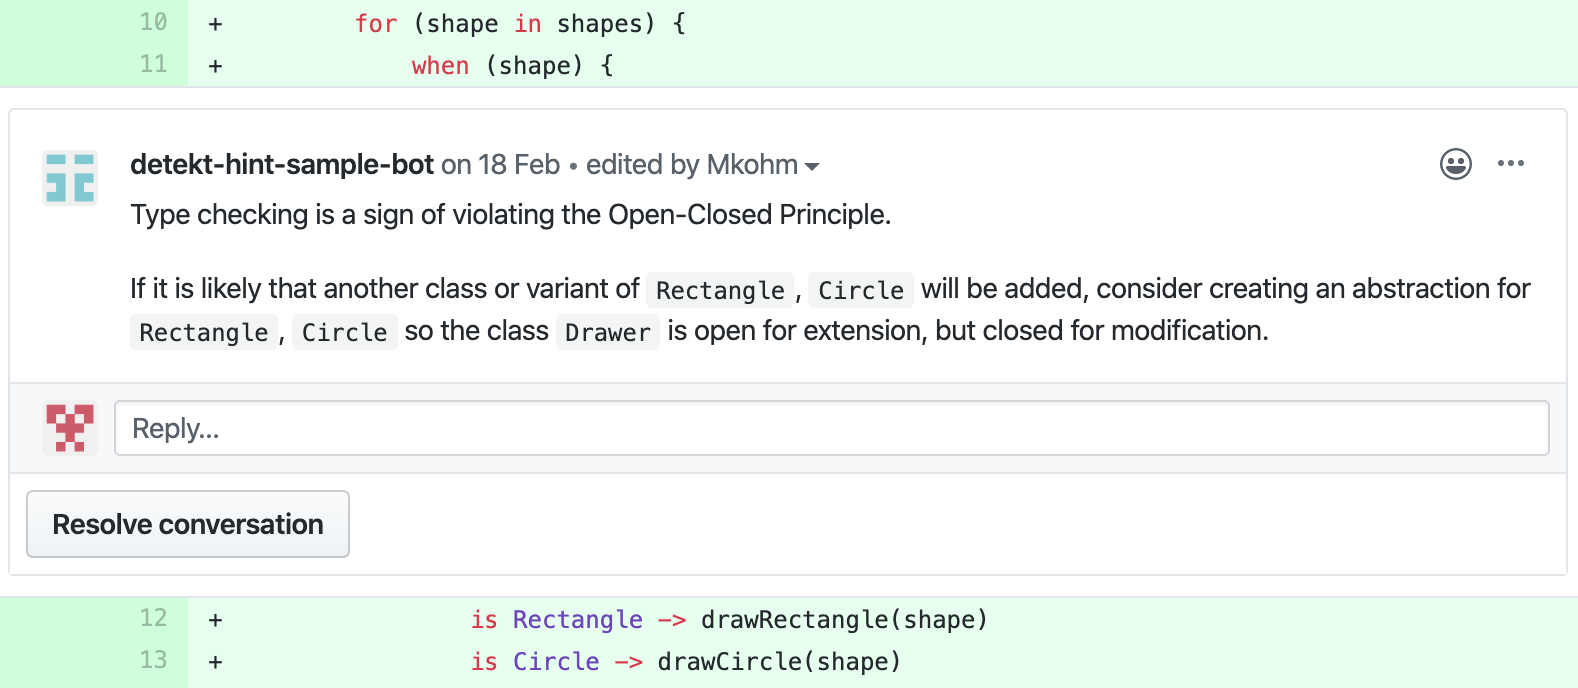
\includegraphics[width=\textwidth]{images/comment_ocp2.png}
    \caption{Screenshot of the horizontal prototype that shows the \gls{ocp} rule, using a simple program for drawing shapes. In this case the rule detected checking of concrete implementations to control flow. The rule suggests creating an abstraction for \texttt{Rectangle}, \texttt{Circle} (e.g an interface \texttt{Shape} with a \texttt{draw} method that all \texttt{Rectangle} and \texttt{Cirle} should implement) such that eventual new shapes added to the program would not need to modify existing code. }
    \label{fig:ocp}
\end{figure}


\begin{figure}[h!]
    \centering
    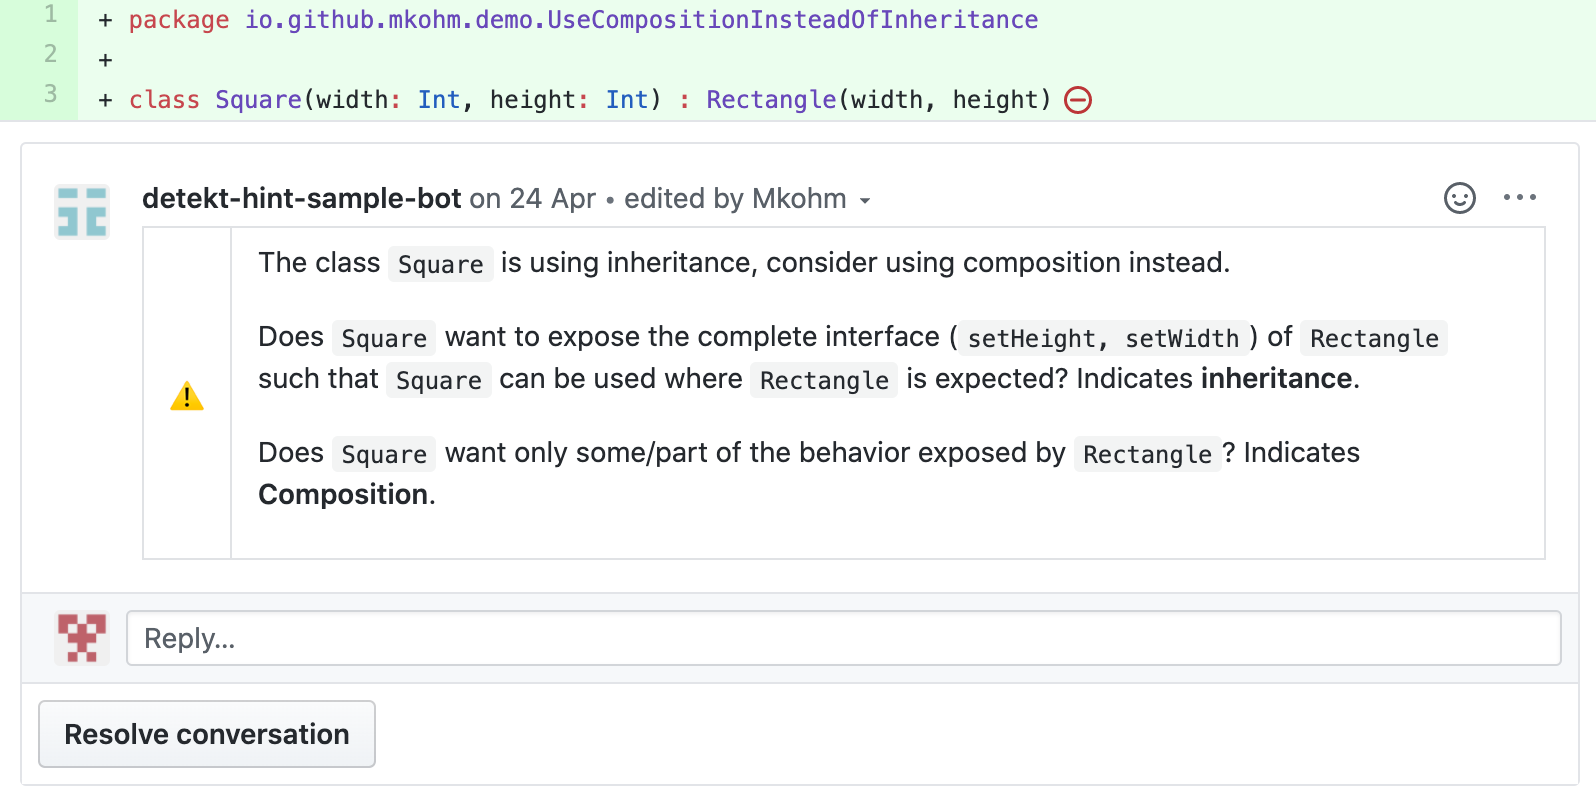
\includegraphics[width=\textwidth]{images/horizontal-prototype-coh.png}
    \caption{Screenshot of the horizontal prototype that shows the \gls{coi} rule. The rule suggests the use of composition instead of inheritance, and helps testing if the classes adheres to the \gls{lsp}. In this case, the classical Square - Rectangle problem is presented. \texttt{Square} should not be derived from \texttt{Rectangle} as it would violate the \gls{lsp}. \texttt{Square} does not functionally behave like \texttt{Rectangle} as squares by definition have the same width and height. \texttt{Rectangle} should have two independent methods for changing its size, but clearly these methods is not appropriate for the \texttt{Square}. }
    \label{fig:liskov}
\end{figure}

\clearpage

\section{Semi-structured interview schema}
\label{semi-structured-interview-schema}
\subsubsection*{Participant number:} What is the number of the participant.
\subsubsection*{Background:} What is the participants background. Experience with software architecture? Knows and uses design principles? Experience with Kotlin?
\subsubsection*{Presentation of rules - For each rule}
\begin{enumerate}
    \item Present the rule. 
    \item Make sure the participant understands the importance of the rule.
    \item When will the rule give a warning?
    \item When will the rule incorrectly give a warning? Will it report false-positives too often? Suggestions on how to reduce the amount?
    \item How much context is needed? Shorter or longer comments? Should include suggestions on possible solutions? Is the comment understandable? Something missing?
\end{enumerate}

\subsubsection*{Other} 
- When reviewing code, what do you think is tedious, and could it be automated?
- Are there any rules/principles missing?

\clearpage
\section{Semi-structured interview results}
\label{horizontal-prototype-interview-results}

\textbf{Participant number:} 1 \newline
\textbf{Background:} Studies computer science at \gls{ntnu} with a specialization in computers and systems software. Has experience with developing apps for iOS and web and back-end development. Interested in Software Architecture and writing software of high quality. \\
\textbf{Experience with design principles:} Some \\\\

\noindent \gls{coi}: Could be useful, but potentially have too many false positives. For testing the participant often creates Mock objects that inherits from the class he wants to Mock, and then overrides methods. The participant think there is too few cases where this rule will be useful. Suggestions: Reduce the amount of positives by disabling checks for classes with names; Mock. User could specify which class names or a pattern to ignore. Should revisit sentence number two about composition, it could be misleading.\\\\

\noindent LCOM1: Very useful because calculating such a value is'nt something you do while coding. Positive that you can change the threshold of the rule. Suggestion: Which fields and methods could i extract? A comment that suggests a solution. \\\\

\noindent LCOM2 (With refactoring visualization): Look more at further analysis to find out what can be extracted. Look into dependencies between function calls as well. Diagram looks cool, but does not give any more value than some plain text explaining what can be extracted. \\\\

\noindent \gls{ocp}: Somewhat useful. Should have a more specific comment saying if you are doing enum switching or instanceOf checking. \\\\

\noindent \gls{isp}: Could be useful. Suggestion to count number of usages of calls in the interface to see which method calls that is not used by any of the classes that implement the interface. \\\\

\noindent Other: Tools for detecting complicated expressions that can be extracted out as a separate method with a descriptive name. Blocks of code should be extracted out as separate methods so that lines of code that belongs together has its own scope. 
\clearpage


% Netlight
\noindent\textbf{Participant number:} 2 \newline
\textbf{Background:} Works as a software developer for Netlight, 2 years of professional developer experience. Experienced with Kotlin development and with architecture and design of software systems.\\
\textbf{Experience with design principles:} Yes \\\\

\noindent \gls{coi}: Positive about the rule, but is concerned about not showing warnings when deriving from third party libraries. This is a case where one also should think about using composition instead of inheritance. Suggests to remove this logic, and instead provide configuration options for packages that should not be reported as violations when derived from.  \\\\

\noindent \gls{lcom}: Nothing special. \\\\

\noindent \gls{ocp}: Useful for both instance of checking and enum switching. Enums in Kotlin are powerful, so switching on them is in many cases not needed and polymorphism is used instead.\\\\

\noindent \gls{isp}: Could be useful. May need to handle TODO's specially. \\\\

\noindent Other: In general positive to the tool, and think it has potential. Good that it is easy to ignore warnings, with just a click. It needs more rules before considering using it. For example including detection of Java anti-patterns and ensuring that Kotlin code is idiomatic. For example static methods and places where data-classes could be used. The tool could be used as "training wheels" in a team, where one gradually could disable more rules to not create unnecessary noise in the development.

\clearpage
\section{Final prototype}
\label{final-artifact}
\begin{figure}[h!]
    \centering
    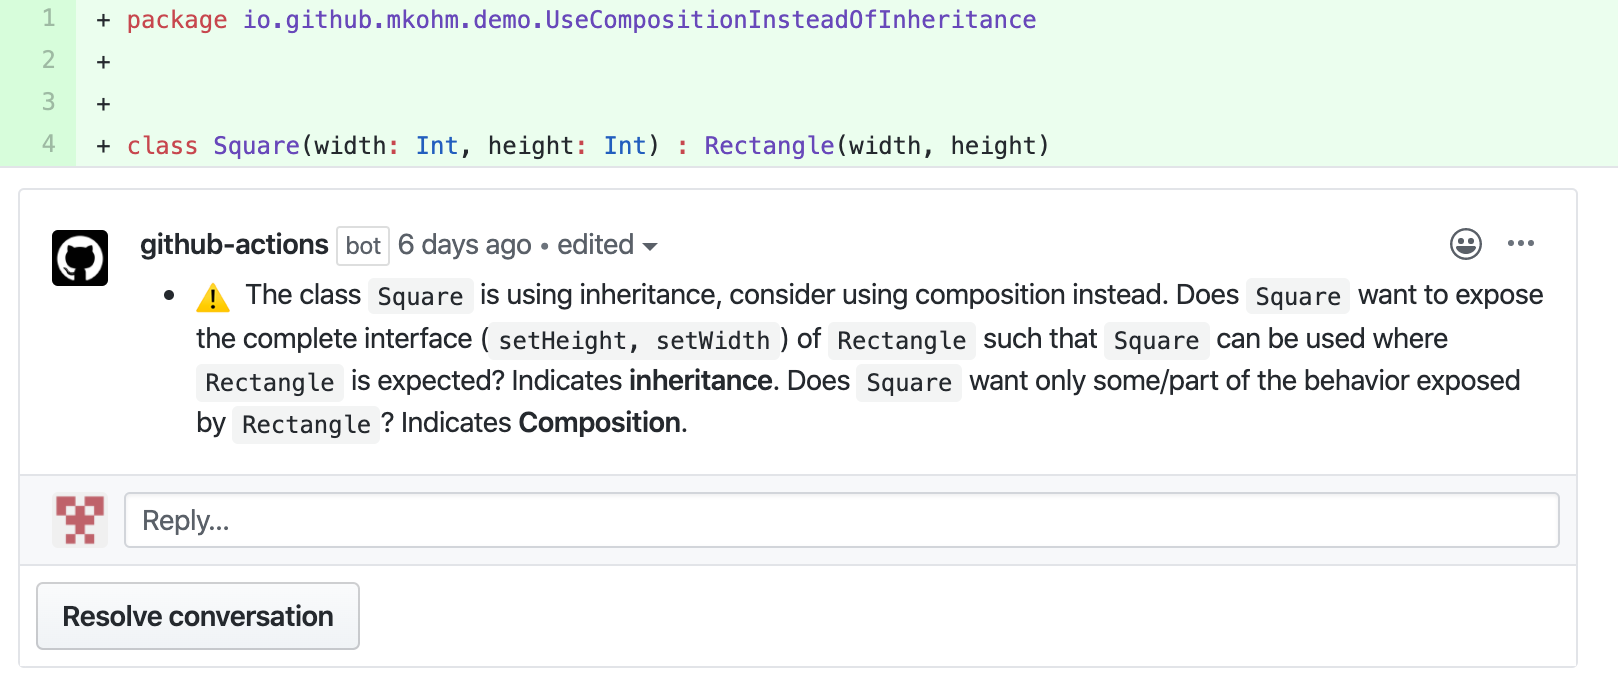
\includegraphics[width=\textwidth]{images/final_coh.png}
    \caption{Screenshot of the final prototype that shows the \gls{coi} rule. The rule suggests the use of composition instead of inheritance, and helps testing if the classes adheres to the \gls{lsp}. In this case, the classical Square - Rectangle problem is presented. \texttt{Square} should not be derived from \texttt{Rectangle} as it would violate the \gls{lsp}. \texttt{Square} does not functionally behave like \texttt{Rectangle} as squares by definition have the same width and height. \texttt{Rectangle} should have two independent methods for changing its size, but clearly these methods is not appropriate for the \texttt{Square}.}
\end{figure}

\begin{figure}[h!]
    \centering
    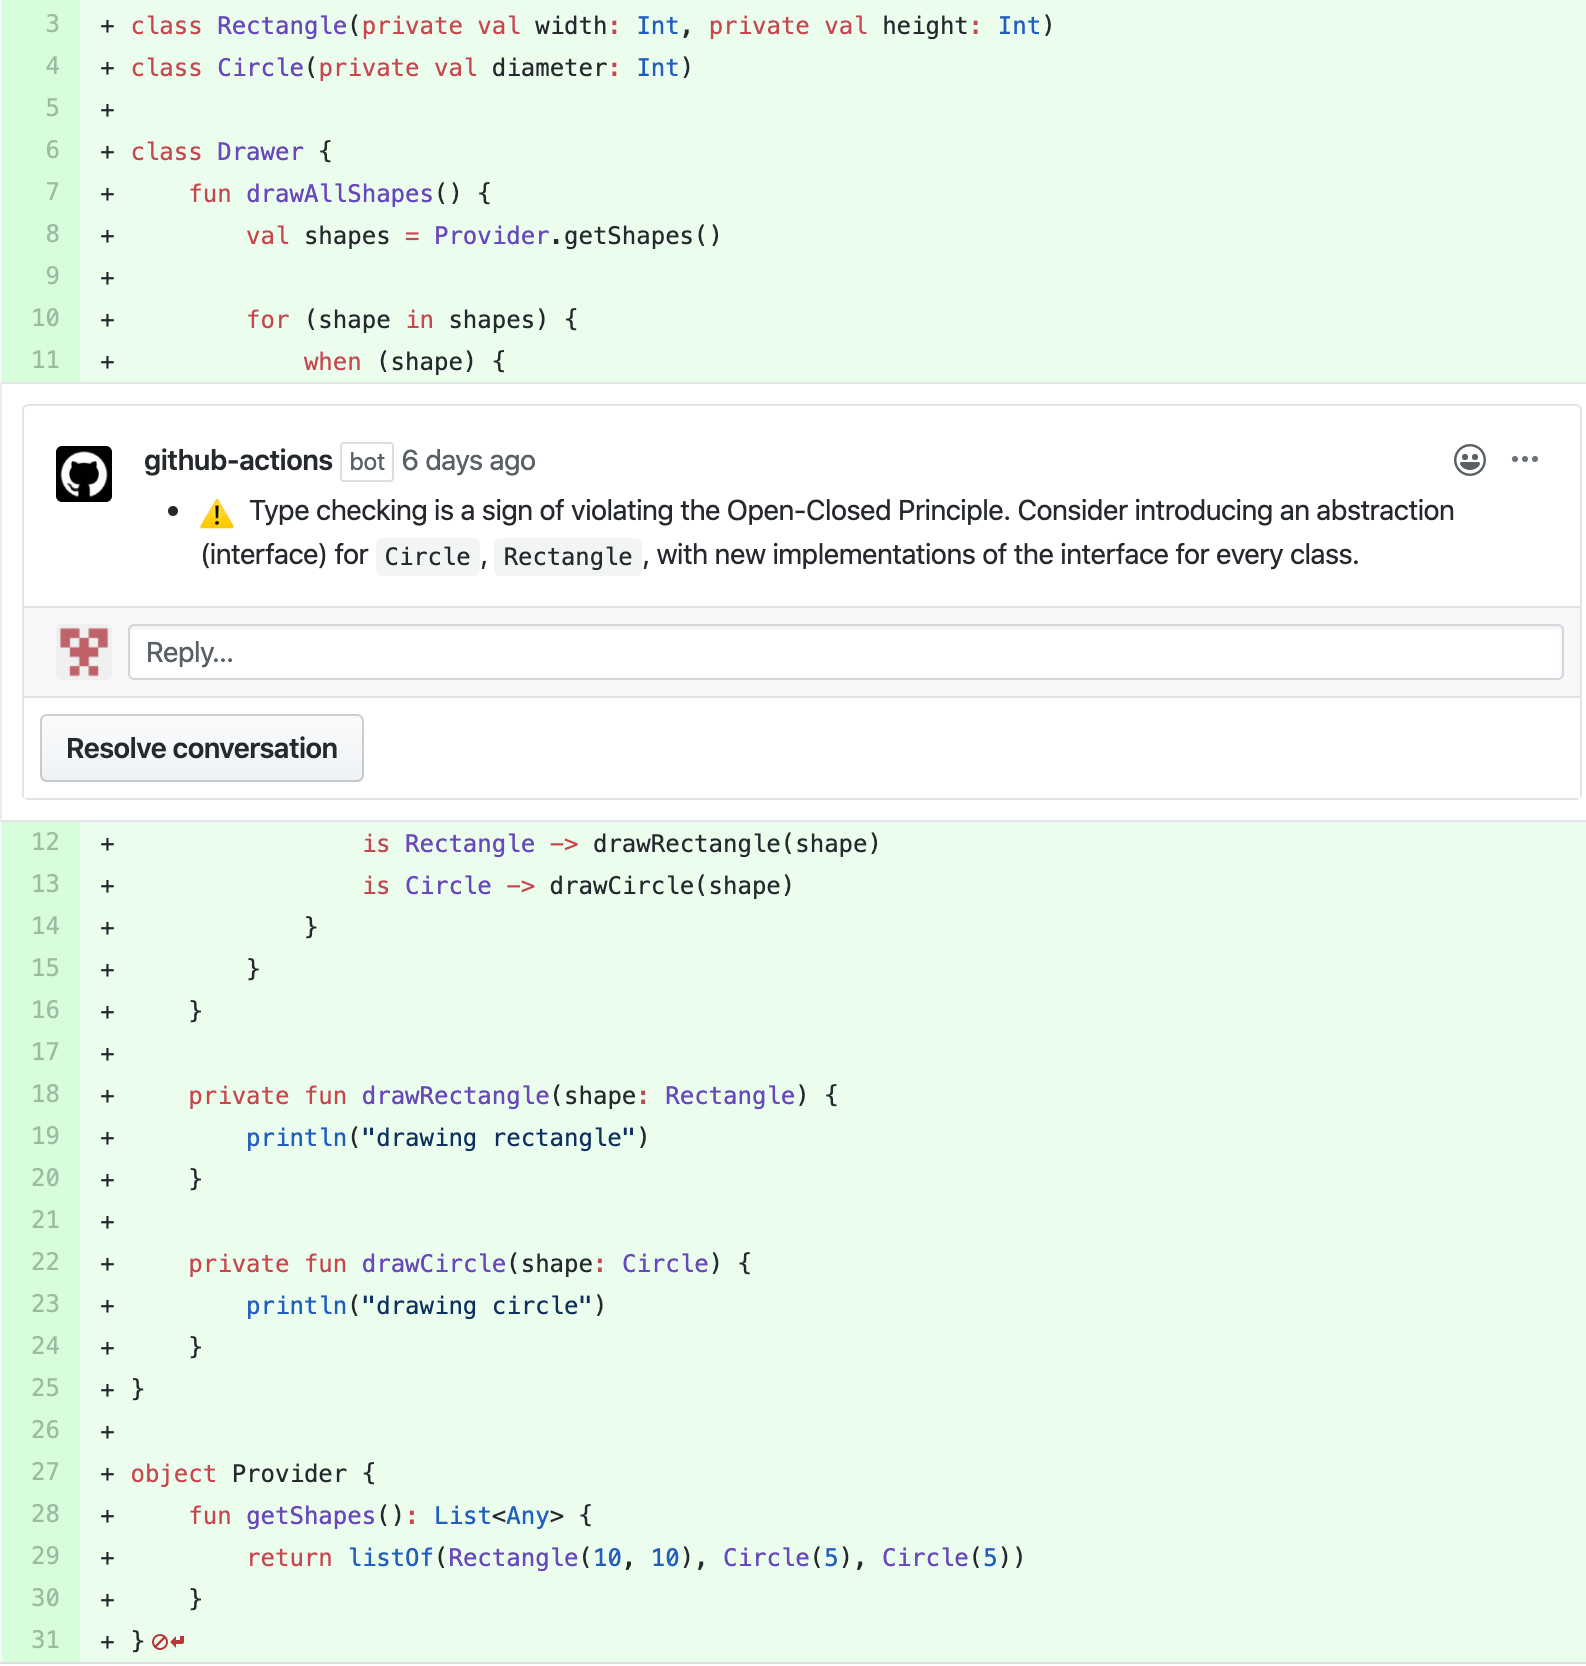
\includegraphics[width=\textwidth]{images/final_ocp.png}
    \caption{Screenshot of the final prototype that shows the \gls{ocp} rule, using a simple program for drawing shapes. In this case the rule detected checking of concrete implementations to control flow. The rule suggests creating an abstraction for \texttt{Rectangle}, \texttt{Circle} (e.g an interface \texttt{Shape} with a \texttt{draw} method that all \texttt{Rectangle} and \texttt{Cirle} should implement) such that eventual new shapes added to the program would not need to modify existing code.}
\end{figure}

\begin{figure}[h!]
    \centering
    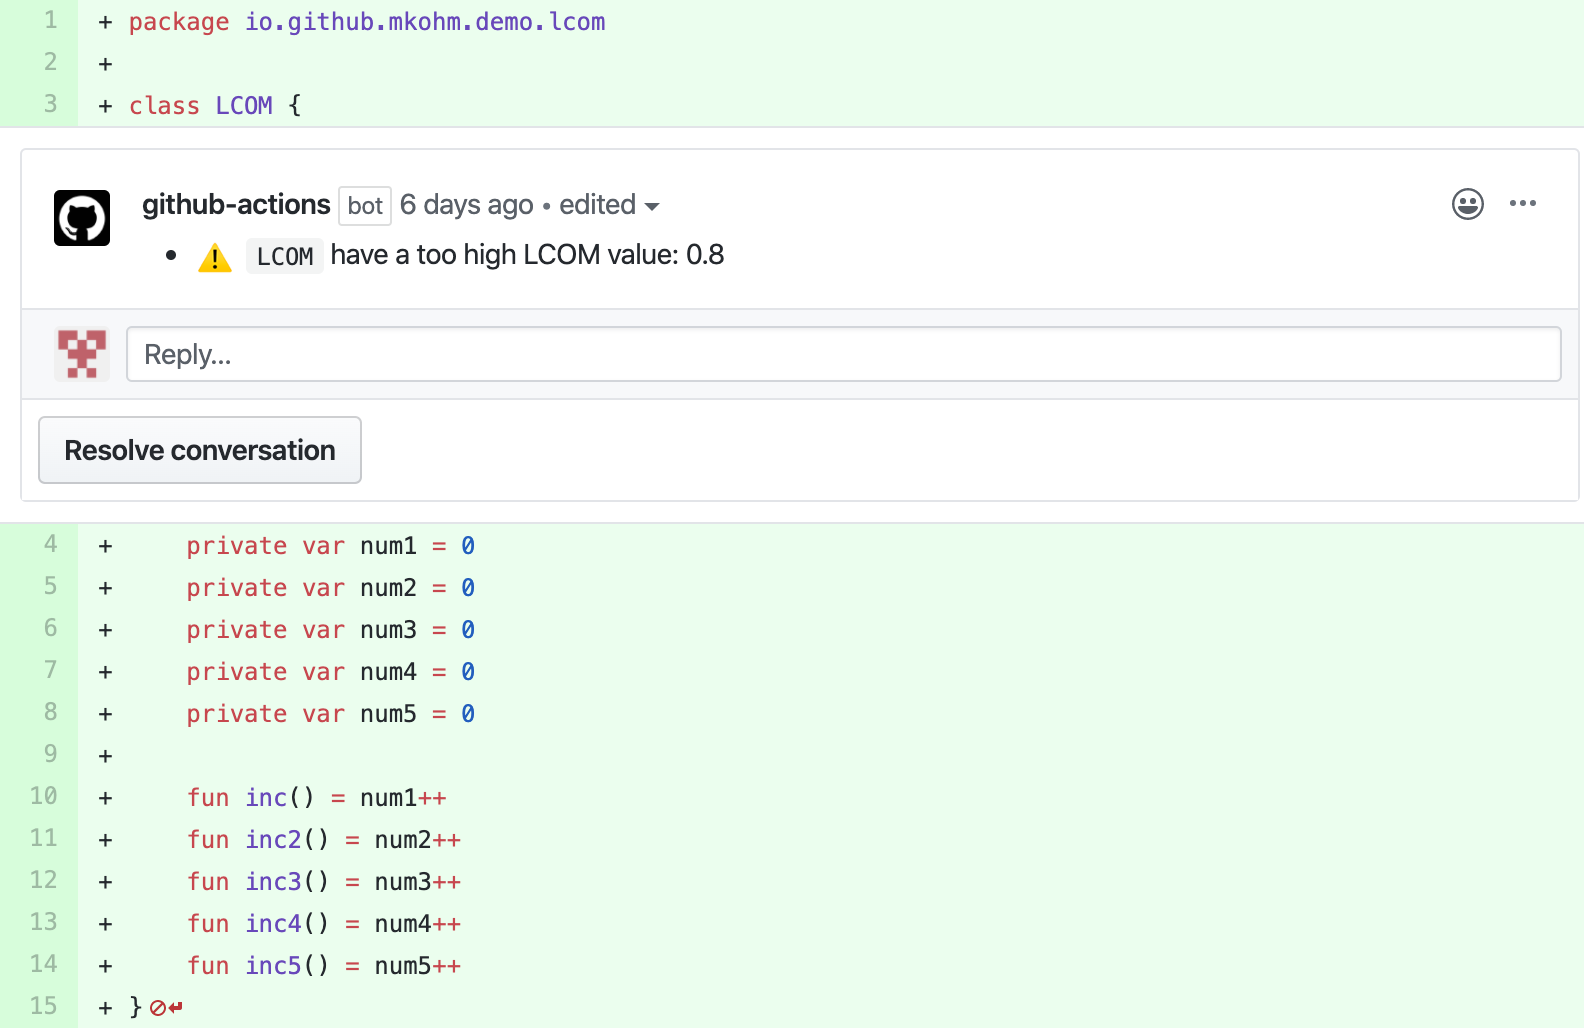
\includegraphics[width=\textwidth]{images/final_lcom.png}
    \caption{Screenshot of the final prototype showing the \gls{lcom} rule. This is an indication of violating the \gls{srp}, due to low cohesion in the class. In this case, each of the methods reference their own field, telling us that there is no relationship between the different methods, and that they don't need to exist in the same class.}
\end{figure}

\begin{figure}[h!]
    \centering
    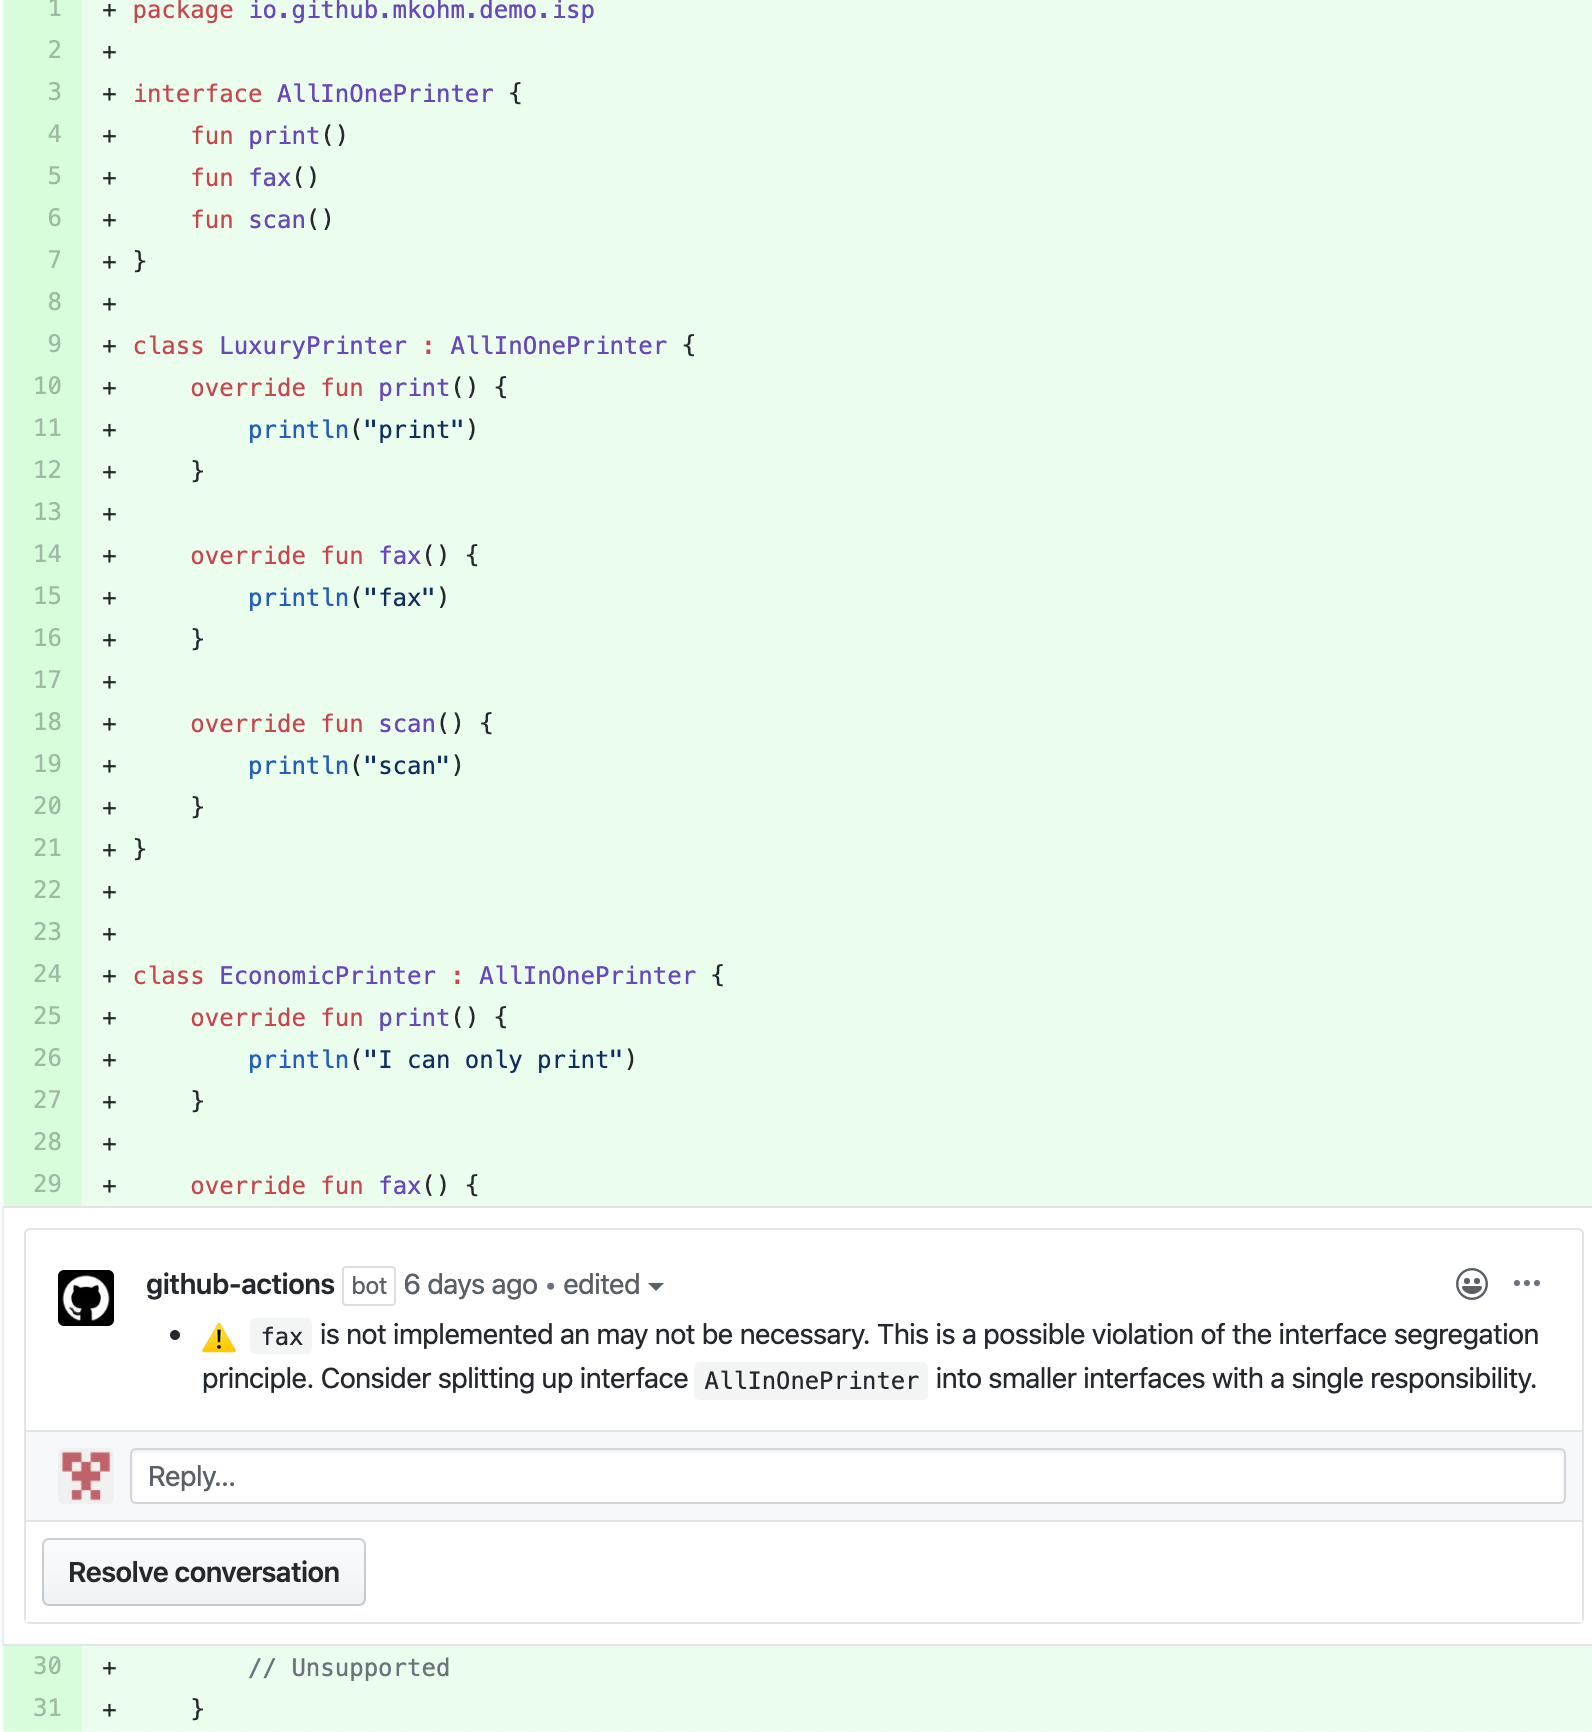
\includegraphics[width=\textwidth]{images/final_isp.png}
    \caption{Screenshot of the final prototype showing the \gls{isp} rule. It has detected an empty method, which is a sign of violating the \gls{isp}. In this case the \texttt{EconomicPrinter} implements methods from \texttt{AllInOnePrinter} which it does not need. A solution would be to define separate interfaces for each of the responsibilities (e.g \texttt{Printable, Faxable, Scanable}) and let the concrete implementations of printers implement the interfaces they need.}
\end{figure}

\end{document}